\documentclass{article}

%%%%%%%%%%%%%%%%%%%%%%%%%%%%%%%%%%%%%%%%%%%%%%%%%%%%%%%%%%%%%%%%%%%%%%%%%%%%%%%%
%% package setup
%%%%%%%%%%%%%%%%%%%%%%%%%%%%%%%%%%%%%%%%%%%%%%%%%%%%%%%%%%%%%%%%%%%%%%%%%%%%%%%%

%\usepackage{enumerate}
\usepackage[shortlabels]{enumitem}
\usepackage{amsfonts, amsmath, amsthm, amssymb, float, mathtools, bbm, etoolbox, xcolor, enumitem}
\usepackage[hyperfootnotes=false]{hyperref}
%\usepackage{soul, matlab-prettifier, multirow, varwidth, array, bm, amssymb}
%\usepackage[all]{xy}
\usepackage[margin=1.3in]{geometry}
%\usepackage{graphicx}
\usepackage{extarrows}
\usepackage{tikz}
\usepackage{tikz-cd}
%\usepackage{bbold}
\usepackage[OT2,T1]{fontenc}
\usepackage{calrsfs}
\usepackage{dsfont}
\usepackage[title]{appendix}
\usepackage{wrapfig}
\usepackage{subcaption}

%%%%%%%%%%%%%%%%%%%%%%%%%%%%%%%%%%%%%%%%%%%%%%%%%%%%%%%%%%%%%%%%%%%%%%%%%%%%%%%%
%% operators and symbols
%%%%%%%%%%%%%%%%%%%%%%%%%%%%%%%%%%%%%%%%%%%%%%%%%%%%%%%%%%%%%%%%%%%%%%%%%%%%%%%%

\newcommand{\define}[4]{\expandafter#1\csname#3#4\endcsname{#2{#4}}}


% operators
\forcsvlist{\define{\DeclareMathOperator}{\mathrm}{}}{Ad, Aut, B, BSD, Char, Cl, Det, End, Frob, Gal, GL, hol, Hom, I, II, III, IV, Id, Ind, Irr, Jac, Ker, Mod, N, new, old, ord,  Perm, PGL, Pic, Proj, PSL, R, Rad, Reg, Rep, res, Res, rk, sign, SL, Smo, SO, Span, Spec, Stab, supp, sw, Sym, Ta, tors, Tr, Trace, un, Vect, contr, Sel, rad, Norm}

%trivial and ell
\newcommand{\trivial}{\mathbbm{1}}
%\renewcommand{\ell}{l}

%mathbb letters 
\forcsvlist{\define{\newcommand}{\mathbb}{b}}{1,A,B,C,D,E,F,G,H,I,J,K,L,M,N,O,P,Q,R,S,T,U,V,W,X,Y,Z, c}

%mathcal letters
\forcsvlist{\define{\newcommand}{\mathcal}{c}}{A,B,C,D,E,F,G,H,I,J,K,L,M,N,O,P,Q,R,S,T,U,V,W,X,Y,Z,a,v, c}

%mathfrak letters
\forcsvlist{\define{\newcommand}{\mathfrak}{f}}{A,B,C,D,E,F,G,H,I,J,K,L,M,N,O,P,Q,R,S,T,U,V,W,X,Y,Z,a,m,n,p,q, g, t, c, f, s}

%overline letters
\forcsvlist{\define{\newcommand}{\overline}{ov}}{H,I,J,K,L,M,N,O,P,Q,R,S,T,U,V,W,X,Y,Z,a,b,c,d,e,f,g,h,i,j,k,l,m,n,o,p,q,r,s,t,u,v,w,x,y,z}

% mathbb
\newcommand{\CC}{\mathbb{C}}
\newcommand{\FF}{\mathbb{F}}
\newcommand{\NN}{\mathbb{N}}
\newcommand{\PP}{\mathbb{P}}
\newcommand{\QQ}{\mathbb{Q}}
\newcommand{\RR}{\mathbb{R}}
\newcommand{\ZZ}{\mathbb{Z}}
\newcommand{\GG}{\mathbb{G}}
\newcommand{\adele}{\mathbb{A}}
\newcommand{\pp}{\mathfrak{p}}
\newcommand{\qq}{\mathfrak{q}}
\newcommand{\rr}{\mathfrak{r}}

% mathfra
%\newcommand{\fg}{\mathfrak{g}}
%\newcommand{\fm}{\mathfrak{m}}

\newcommand{\norm}[1]{\left\lVert#1\right\rVert}
\newcommand{\hatv}[1]{\overset{\vee}{\mathstrut#1}}
\newcommand{\legendre}[2]{\ensuremath{\left( \frac{#1}{#2} \right) }}
\newcommand{\repnorm}[1]{\fN_{\bQ(#1) / \bQ}(#1)}
\newcommand{\fieldnorm}[1]{N_{\bQ(#1) / \bQ}(\bQ(#1)^{\times})}
\newcommand{\defeq}{\mathrel{\mathop:}=} 
\newcommand{\C}{\hat{C}}

% Structures
\def\set#1{\left\{#1\right\}}
%\def\sets#1#2{\left\{\left.#1\ \right\vert#2\right\}}
\def\rbr#1{\left(#1\right)}
\def\ang#1{\left\langle#1\right\rangle}
\def\n#1{\left\lvert#1\right\rvert}
\def\nn#1{\left\lVert#1\right\rVert}
\def\eq#1{\begin{equation}#1\end{equation}}
\def\ov#1#2{{\substack{#1\\#2}}} % #1 over #2

% Symbols
\def\mto{\mapsto}
\def\emb{\hookrightarrow}
\def\es{\emptyset}
\def\bs{\backslash}
\def\cupp{\smallsmile}
\def\surj{\twoheadrightarrow}

% floor and ceiling
\DeclarePairedDelimiter\ceil{\lceil}{\rceil}
\DeclarePairedDelimiter\floor{\lfloor}{\rfloor}

\DeclareMathOperator{\Ima}{Im}
%\linespread{1.5}

\theoremstyle{plain}
\newtheorem{thm}{Theorem}[section]
\newtheorem{question}[thm]{Question}
\newtheorem{prop}[thm]{Proposition}
\newtheorem{condition}[thm]{Condition}
\newtheorem{lemma}[thm]{Lemma}
\newtheorem{cor}[thm]{Corollary}
\newtheorem{algo}[thm]{Algorithm}
\theoremstyle{definition}
\newtheorem{defn}[thm]{Definition}
\newtheorem{notn}[thm]{Notation}
\newtheorem{rem}[thm]{Remark}
\newtheorem{example}[thm]{Example}
\newtheorem{exercise}[thm]{Exercise}
\newtheorem{examples}[thm]{Examples}
\newtheorem{fact}[thm]{Fact}

\newtheorem{conj}[thm]{Conjecture}
\newtheorem*{conj*}{Conjecture}
\newtheorem{notation}[thm]{Notation}
\newtheorem*{thm*}{Theorem}

%Sha:
\usepackage[OT2,T1]{fontenc}
\DeclareSymbolFont{cyrletters}{OT2}{wncyr}{m}{n}
\DeclareMathSymbol{\Sha}{\mathalpha}{cyrletters}{"58}
%end of Sha

%\DeclareSymbolFont{cyrletters}{OT2}{wncyr}{m}{n}
%\DeclareMathSymbol{\Sha}{\mathalpha}{cyrletters}{"58}

%\DeclareMathAlphabet{\pazocal}{OMS}{zplm}{m}{n}

\title{Arithmetic Applications of Artin Twist and BSD}
\author{Edwina Aylward, Albert Lopez Bruch}

\begin{document}
	\maketitle
	\pagenumbering{arabic}
	\newpage
	\tableofcontents
	\newpage

\section*{Introduction}
In this report we study a method proposed in \cite{DEW1} for forcing points of infinite order on elliptic curves over finite extensions $F / \bQ$. 

\subsection*{Notation}
We use the following notation for characters:

\bigskip

\begin{tabular}{l | l}
    $R_(G)$ & the representation ring of $G$, \\
    $R_{\bQ}(G)$ & the rational representation ring of $G$, \\
    $\Perm(G)$ & the ring of virtual permutations of $G$, \\
    $\Char_{\bQ}(G)$ & the ring of rationally-valued characters of $G$,\\
    $\Irr(G)$ & the set of characters of complex irreducible representations of $G$, \\
    %$\Irr_{\bQ}(G)$ & the set of characters of $\bQ$-irreducible representations of $G$, \\ 
    $\bQ(\rho)$ & the field of character values of a complex character $\rho$ of $G$, \\
    $C(G)$ & the finite abelian group $\Char_{\bQ}(G) / \Perm(G)$, \\ 
    %$m(\rho)$ & the Schur Index of an irreducible complex character $\rho$ over $\bQ(\rho)$, \\
    \\
    $H^{x}$ & $= xHx^{-1}$  for $H \leq G$ a subgroup of a group $G$ and $x \in G$,
\end{tabular}
\vspace{2em}

Given an elliptic curve $E / \bQ$ and a number field $F$, we define

\[ C_{E / F} = \prod_v c_v(E / F) \left| \frac{\omega}{\omega_v^{\min}} \right|_v. \]
The product is taken over the finite places of $F$, $\omega$ is a global minimal differential for $E / \bQ$, and $\omega_v^{\min}$ is a minimal differential at $v$. In terms of minimal discriminants, if $E$ is of the form
\[ y^2 + a_1 x y + a_3 y = x^3 + a_2 x^2 + a_4 x + a_6 \]
with minimal discriminant $\Delta_E$ and $\omega = \frac{dx}{2 y + a_1 x + a_3}$, then
\[ \left| \frac{\omega}{\omega_v^{\min}} \right|_v^{-12} = \left| \frac{\Delta_E}{\Delta_{E, v}^{\min}} \right|_v . \]



\newpage
\section{Norm relations}
As observed in the introduction, we will be considering Artin representations over $\bQ$ that factor through finite Galois groups $G = \Gal(F / \bQ)$. Our methods in this report apply the theory of finite group representations to the study of elliptic curves over finite Galois extensions. This section introduces some representation-theoretic concepts that we will apply in later sections. 

The first two subsections discuss rational representations of $G$, and writing these as a sum of virtual permutation representations.
In the third subsection, we consider functions defined on subgroups of $G$, corresponding to subfields of $F / \bQ$. Our main example of interest is the function sending $H \mapsto C_{E / F^H}$ for $H \leq G$ \footnote{this is the fudge factor that appears in the BSD quotient for $E / F^H$}. We also describe \textit{$D$-local functions}, which are functions that depend on a decomposition group, borrowing definitions that appear in \cite[Section 2.iii]{reg-const}.

We have attempted to make this first section mainly representation-theoretic, in case the results within can be applied in other contexts.

\subsection{Rational characters and permutation representations}\label{rep}

\begin{defn} 
    Let $G$ be a finite group, $K$ a field of characteristic zero.
\begin{enumerate}
    \setlength\itemsep{0em}
    \item A \textbf{representation} of $G$ over $K$ is a group homomorphism $\rho \colon G \to \GL(V)$ where $V$ is a $K$-vector space.
    \item  Associated to a representation $\rho$ is a \textbf{character} $\chi \colon G \to K^{\times}$, defined by letting $\chi(g) = \Tr \rho(g)$ for $g \in G$. 
\end{enumerate}
\end{defn}

If we don't specify the field a representation is defined over, assume it is defined over $\bC$. For complex representations, $\rho$ is determined by its character; if $\rho$, $\rho'$ are representations with identical characters, then $\rho$ and $\rho'$ are isomorphic as representations (cf. \cite[Chapter 2, \S 2.3]{Serre}). 

%\begin{defn}\label{rep-ring}
%Let $\chi_1, \ldots,  \chi_h$ be the distinct characters of the complex irreducible representations of $G$, where $h = \#$ conjugacy classes of $G$. 
%Then the \textbf{representation ring} of $G$ is 
%\[ \R(G) = \bZ \chi_1 \oplus \cdots \oplus \bZ \chi_h .\]
%We can also view this as the Grothendieck group of the category of finitely generated $\bC[G]$-modules.
%\end{defn}
%Since we take differences of characters in $\R(G)$, we call elements of $\R(G)$ \textbf{virtual representations}. 

Let $K$ be a number field. Denote by $\R_K(G)$ the group generated by characters of the representations of $G$ over $K$. A representation of $G$ is then defined over $K$ if and only if its character is in $\R_K(G)$ (\cite[Proposition 33]{Serre}).
$\R_K(G)$ is a subring of $\R_{\bC}(G)$, where $\R_{\bC}(G)$ is finitely generated by $\Irr(G)$; the irreducible characters of $G$ over $\bC$.
When $K = \bQ$ this is called the \textbf{rational representation ring}.
The characters of the distinct irreducible representations of $G$ over $K$ form an orthogonal basis of $\R_K(G)$ with respect to the usual inner product of characters of $G$ (\cite[Proposition 32]{Serre}).
Let $m$ be the exponent of $G$. If $K$ contains the $m$-th roots of unity, then $\R_K(G) = \R_{\bC}(G)$ (\cite[Theorem 24]{Serre}). This implies every representation of $G$ can be realized over such $K$. 
\vspace{1em}

%The rank of $R_K(G)$ is discussed in {\color{red} Serre 12.4}.
Let $\Perm(G)$ be the ring of virtual permutation representations of $G$ (i.e. the ring generated by the characters of $\bC[G / H] = \Ind_{H}^G \trivial$ for $H \leq G$). Let $\Char_{\bQ}(G)$ be the ring of rationally valued characters of $G$. Then we have inclusions 
\[ \Perm(G) \to \R_{\bQ}(G) \to \Char_{\bQ}(G). \]
Each of these groups have equal $\bZ$-rank, equal to the number of conjugacy classes of cyclic subgroups of $G$ (\cite[Chapter 13, \S13.1]{Serre}). Moreover the cokernels of these maps are finite.

\begin{defn}\label{rho-norm}
    Let $\rho$ be a representation of $G$. We define the norm of $\rho$, denoted $\repnorm{\rho}$, by 
    \[
    \repnorm{\rho} \defeq \sum_{\fg \in \Gal(\bQ(\rho)/\bQ)}  \rho^\fg \quad,
    \]
    where $\bQ(\rho)$ is the abelian extension of $\bQ$ generated by $\{ \Tr \rho(g) \colon g \in G \}$, and $\rho^\fg$ is the representation of $G$ such that $\Tr \rho^{\fg}(g) = \fg(\Tr \rho(g))$ for $g \in G$. 
\end{defn}

It's clear that $\Char_{\bQ}(G)$ is generated by the characters of $\repnorm{\rho}$ as $\rho$ ranges over the complex irreducible representations of $G$. Indeed, if a representation has a rationally valued character, then any complex irreducible constituent must occur along with all its Galois conjugates with equal multiplicity.

\begin{rem}
This is not additive, i.e. one does not have \[\repnorm{\rho + \tau} = \repnorm{\rho} + \repnorm{\tau}. \] 
This does hold when $\bQ(\rho) = \bQ(\tau)$. 
\end{rem}

\begin{example}
    Let $G = C_p$ and $\psi_p$ a character of order $p$. Then $\bQ(\psi_p) = \bQ(\zeta_p)$ and $\repnorm{\psi_p}$ is the sum over the $p - 1$ non-trivial characters of $G$. But $\repnorm{\psi_p + \trivial} = \trivial^{\oplus (p - 1)} + \repnorm{\psi_p} \not= \repnorm{\trivial} + \repnorm{\psi_p}$.
\end{example}

%Conversely,  Therefore our map $R(G) \to \Char_{\bQ}(G)$ is surjective.

%Such a character may not be in $R_{\bQ}(G)$, however. That is, it has rational character, but the corresponding representation cannot be realized over $\bQ$. The quotient $\Char_{\bQ}(G) / R_{\bQ}(G)$ is the study of Schur indices.  If $\rho \in R(G)$ is an irreducible representation, the \textbf{Schur index} is the smallest integer $m(\rho)$ such that 
%\[ \sum_{\sigma \in \Gal(\bQ(\rho)/\bQ)}m(\rho) \cdot \rho^\sigma \quad \in R_{\bQ}(G). \]

\begin{rem}\label{image-of-burnside}
The group $$\C(G) \defeq \frac{\Char_{\bQ}(G)}{\Perm(G)}$$ is a finite abelian group, of exponent dividing $|G|$ (this follows from Artin's induction theorem, \cite[Theorem 17]{Serre}). The study of this group is quite subtle. For us, it's enough to know that given a representation $\rho$ of $G$, there exists a minimum integer $m$, depending on $\rho$ and dividing $|G|$, such that 
\[ \repnorm{\rho}^{\ \oplus m } = \bigoplus_i \Ind_{H_i}^G \trivial \ominus \bigoplus_j \Ind_{H_j'}^{G} \trivial \]
for some subgroups $H_i$, $H_j' \leq G$, i.e. that the character of $\repnorm{\rho}^{\ \oplus m }$ is in $\Perm(G)$. This minimum integer $m$ is the order of the character of $\repnorm{\rho}$ in $\C(G)$. 
\end{rem}
%Thus, we have a map $\Irr(G) \to \Perm(G)$. We extend this additively to a map $R(G) \to \Perm(G)$.
\begin{example}
If $G = C_n$ then $\C(G)$ is trivial (see Example \ref{cyclic-relns}). $\C(G)$ is also trivial for the symmetric groups $G = S_n$. 
\end{example}

 \begin{example}
    $G = Q_8$, the quaternion group, has $\C(G) = \bZ / 2 \bZ$. Let $\rho$ be the faithful irreducible representation of $G$ of dimension $2$. Its character $\chi$ is rational and one has 
    \[ \rho^{\oplus 2} = \Ind_{C_1}^G \trivial \ominus \Ind_{C_2}^G \trivial, \]
    but one cannot write $\rho$ as a virtual permutation representation ($\chi$ has Schur index $2$ so $\chi \not\in \R_{\bQ}(G)$).  
 \end{example}

%\begin{notn}
%For $\rho \in R_{\bC}(G)$ an irreducible character let 
%\[  \repnorm{\rho} = \sum_{\sigma \in \Gal(\bQ(\rho)/\bQ)}m(\rho)\cdot \rho^\sigma \quad \in R_{\bQ}(G) , \]
%where $m(\rho) \in \bZ$ is the Schur index of $\rho$.
%\end{notn}
%Then $\repnorm{\rho}$ is the character of an irreducible rational representation. Every irreducible rational representation can be obtained this way. We can extend this map additively to a surjective map $R_{\bC}(G) \to R_{\bQ}(G)$. 

%Let $\overline{R_K(G)}$ be the subring of elements of $R(G)$ which have values in $K$. Then $R_K(G) \subset \overline{R_K(G)}$ and this inclusion is of finite index. 
%Given a character $\chi$ of $G$, let $\bQ(\chi)$ be the smallest subfield of $\bC$ containing $\{ \chi(g) \mid g \in G \}$.
%Let $R_{\bC}(G)$ denote the ring of characters of complex representations of $G$. The number of complex irreducible representations of $G$ is equal to the number of conjugacy classes of $G$. Let $R_{\bQ}(G)$ be the ring of characters of rational valued representations of $G$.
%The number of irreducible $\bQ G$-representations up to isomorphism is equal to the number of conjugacy classes of cyclic subgroups of $G$. %(\cite[$\mathsection 13.1$, Cor. 1]{Serre})
%Induction, Restriction\dots
%\begin{thm}[Mackey Decomposition] 
%\end{thm} 

\subsection{The Burnside ring and relations for permutation representations}

Let $G$ be a finite group. Recall that there is a bijection  
\[ \{ \text{transitive finite }G\text{-sets } X  \text{ up to isomorphism}\}\leftrightarrow  \{ \text{subgroups } H \leq G \text{ up to conjugacy} \} \] 
given by sending a transitive finite $G$-set $X$ to $H = \Stab_{G}(x)$ for some $x \in X$.  The action of $G$ on $X$ is equivalent to the action of $G$ on $G / H$. 

\begin{defn}\label{burnside}
Let $[X]$ denote the isomorphism class of a $G$-set $X$. 
The \textbf{Burnside ring} $\B(G)$ is the free abelian group on isomorphism classes of finite $G$-sets, modulo the relations  $[S] + [T] = [S \sqcup T]$ for $S$, $T$ finite $G$-sets. This is a ring; multiplication is given by $[S] \cdot [T] = [S \times T]$.
\end{defn}

We only need that $\B(G)$ is a group, and do not use its multiplicative structure. $\B(G)$ is generated by $\{ [X] \colon X \text{ finite transitive } G\text{-set}\}$. Using the identification of finite transitive $G$-sets with subgroups of $G$, we write elements of $\B(G)$ as $\sum_i n_i H_i$ for $n_i \in \bZ$, $H_i \leq G$. 

\begin{defn}
    Given a $G$-set $X$, one obtains a representation of $G$ by considering its permutation representation $\bC[X]$. We extend this to $\B(G)$; given $\Theta  = \sum_i n_i H_i \in \B(G)$, define 
    \[ \bC[G / \Theta ] = \sum_i n_i \Ind_{H_i}^G \trivial. \]
    Let $\chi_{\bC[G / \Theta]}$ be the character of $\bC[G / \Theta]$. Then  $\Theta \mapsto \chi_{\bC[G / \Theta]}$ defines a homomorphism $\B(G) \to \Perm(G)$.
\end{defn}

\begin{defn}
If $\bC[G / \Theta] = 0$ as a virtual permutation representation (i.e. $\chi_{\bC[G / \Theta]} = 0$), then $\Theta$ is called a  \textbf{Brauer relation}.
\end{defn}

Non-trivial Brauer relations are instances of non-isomorphic $G$-sets giving rise to isomorphic permutation representations. 

\begin{example}
    The irreducible representations of $G = S_3$ are the trivial representation $\trivial$, the sign representation $\epsilon$ and the $2$-dimensional representation $\rho$.
    We have
    \begin{table}[H]
        \centering
    \begin{tabular}{l l l l l l l}
        $\bC[G / C_1]$ & $=$ & $\trivial \oplus \epsilon \oplus \rho^{\oplus 2},$ & $\qquad$ &
        $\bC[G / C_2]$ & $=$ & $\trivial \oplus \rho,$\\ 
        $\bC[G / C_3]$ & $=$ & $\trivial \oplus \epsilon,$ & $\qquad$ &
        $\bC[G / G]$ & $=$ & $\trivial.$  
    \end{tabular}
\end{table}
    Then $\Psi = C_1  - 2 C_2 - C_3 + 2S_3$ is the unique Brauer relation for $G$.
\end{example}

\begin{example}\label{cyclic-no-brauer}
Cyclic groups have no Brauer relations. Indeed, if $G = C_n$, the $\bZ$-rank of $\Perm(G)$ is the number of cyclic subgroups of $C_n$, i.e the number of subgroups of $C_n$, which is the $\bZ$-rank of $\B(G)$. Hence the rank of the kernel of the map $\B(G) \to \Perm(G)$ is zero.
\end{example}

In the last section, we described how to obtain a virtual permutation representation from an arbitrary representation of $G$. We are interested in when this is an image of an element from the Burnside ring.

\begin{defn}
Let $\rho$ be a representation of $G$.    
We call $\Theta = \sum_i n_i H_i \in \B(G)$ a \textbf{$\rho$-relation} if $\bC[G / \Theta] \simeq \repnorm{\rho}^{\ \oplus m}$, for some $m \geq 1$.
\end{defn}

If $D \leq G$, then one can pass from virtual permutation representations of $G$ to virtual permutation representations of $D$ via restriction, and in the other direction via induction. We define analogous maps for the Burnside ring.    

\begin{defn}
    For $D \leq G$, define maps $\Res_D \colon \B(G) \to \B(D)$ and $\Ind_D \colon \B(D) \to \B(G)$ by
    \[  \Res_D H = \sum_{x \in H \backslash G / D} D \cap H^{x^{-1}}, \qquad \quad \Ind_D H = H. \]
    These correspond to the representation theory side, where $\Res_D \Ind_{H}^G \trivial = \sum_{x \in H \backslash G / D} \Ind_{D \cap H^{x^{-1}}}^D \trivial$ (Mackey's decomposition, cf. \cite[Chapter 7, \S 7.3]{Serre}, $H^{x^{-1}} = x^{-1}H x$), and $\Ind_{D}^G\Ind_{H}^D \trivial = \Ind_{H}^G \trivial$.
\end{defn}
%\begin{rem}
%If such a relation exists, then $m$ is a multiple of the order of $\repnorm{\rho}$ in $C(G)$. Note that if $\Theta$ is a $\rho$-relation and $\Psi \in B(G)$ is a Brauer relation, then $\Theta + \Psi$ is also a $\rho$-relation. It follows that for a fixed $m \geq 1$, if $\repnorm{\rho}^{\oplus m} \in \Perm(G)$ then there are $\#$(Brauer relations of $G$) $+ 1$ elements $\Theta \in \B(G)$ with $\bC[G / \Theta] = \repnorm{\rho}^{\oplus m}$.
%\end{rem}

The following are some elementary properties of these relations:

\begin{prop} Let $\rho$ be a representation of $G$, $\Theta = \sum_i n_i H_i \in \B(G)$ a $\rho$-relation. Then,
    \begin{enumerate}
        \item $n \Theta$ is a $\rho$-relation for all $n \geq 1$.
        \item $\bC[G / \Theta] \simeq \repnorm{\rho}^{\oplus m}$ where $m$ is a multiple of the order of the character of $\repnorm{\rho}$ in $\C(G)$.
        \item If $\Psi \in B(G)$ is a Brauer relation, then $\Theta + \Psi$ is also a $\rho$-relation. 
        \item For a fixed $m \geq 1$, if $\repnorm{\rho}^{\oplus m}$ is a virtual permutation representation then there are $\#$(Brauer relations of $G$) $+ 1$ elements $\Theta \in \B(G)$ with $\bC[G / \Theta] = \repnorm{\rho}^{\oplus m}$.
        
        \item (Projection) If $N \trianglelefteq G$ then $(N \cdot \Theta) / N = \sum_i n_i N H_i / N$ is a $\rho^N$-relation, viewing this relation as an isomorphism of representations of $G / N$.
        \item (Restriction) For $D \leq G$, $\Res_D \Theta$ is a $\Res_D \rho$-relation.
    \end{enumerate}
\end{prop}

\begin{proof}
    All but (5) are clear. For (5), observe that for $H \leq G$, $\bC[G / H]^N \simeq \bC[G / NH]$ as $G$-representations (see proof of \cite[Theorem 2.8]{reg-const}). We also need to show that $\repnorm{\rho}^N \simeq \repnorm{\rho^N}^{\oplus k}$ for some $k \geq 1$. This is the case; 
    $$\repnorm{\rho}^N = \left(\bigoplus_{\fg \in \Gal(\bQ(\rho) / \bQ)} \rho^{\fg} \right)^N \simeq 
    \bigoplus_{\fg \in \Gal(\bQ(\rho) / \bQ)} (\rho^{\fg})^N \simeq \bigoplus_{\fg \in \Gal(\bQ(\rho) / \bQ)} (\rho^N)^{\fg} = \repnorm{\rho^N}^{\oplus k},$$
    where $k = [ \bQ(\rho) : \bQ(\rho^N)]$. 
\end{proof}


\begin{example}\label{cyclic-relns}
    Let $G = C_n$. For each $d \mid n$, let $\chi_d = \repnorm{\varphi_d}$, where $\varphi_d$ is an irreducible complex character of $G$ with field of values $\bQ(\zeta_d)$ and kernel of index $d$.
    Then $\{ \chi_d \colon d\mid n \}$ form an orthogonal basis for the irreducible rational-valued representations of $G$ {\color{red} cite Serre exercise}. Since $C_{n / d} \trianglelefteq G$, $\Ind_{C_{n/ d}}^G \trivial$ is the direct sum of irreducible complex representations of $G$ containing $C_{n / d}$ in their kernel. Thus, $\Ind_{C_{n/ d}}^G \trivial \simeq \sum_{d' \mid d} \chi_{d'}$. Applying M\"{o}bius inversion, we obtain a $\varphi_d$-relation for each $d \mid n$:
    \[ \chi_d = \sum_{d' \mid d} \mu(d / d') \cdot \Ind_{C_{n/ d}}^G \trivial. \]
    Note that this is the only way of writing $\chi_d$ as a sum of permutation representations, since cyclic groups have no Brauer relations (Example \ref{cyclic-no-brauer}). Similarly, there is a unique $\Theta \in B(G)$ such that $\bC[G / \Theta] \simeq \chi_d^{m}$ for all $m \geq 1$.
    \end{example}

\subsection{Functions on the Burnside ring and norm relations}\label{sec-norm-rels}

In this section, consider $f \colon \B(G) \to A$ a multiplicative function with $f(\sum_i n_i H_i) = \prod_i f(H_i)^{n_i}$ where $A$ is an abelian group. As in \cite{reg-const}, we say that $f$ is \textbf{representation theoretic} if $f$ is trivial on Brauer relations. This implies that for a $G$-set $X$, $f$ only depends on the representation $\bC[X]$. 
%In other words, there exists a map $g \colon \R(G) \to A$ such that $f(H) = g(\bC[G / H])$ for all $H \leq G$. 

\begin{example}
  Let $\lambda \in \bR^{\times}$ and consider the function $H \mapsto \lambda^{[G : H]}$. This is trivial on Brauer relations;  if $\sum_i n_i H_i$ is a Brauer relation then $\lambda^{\sum_i n_i [G : H]} = \lambda^{\dim( \oplus_i \bC[G / H_i]^{\oplus n_i})} = 1$.
\end{example}

Let $\rho$ be a representation of $G$. Let $\Theta \in \B(G)$ be a $\rho$-relation, with $\bC[G / \Theta] \simeq \repnorm{\rho}^{\oplus m}$. In the introduction, {\color{red} add motivation}

\begin{defn}
Let $\rho$ be a representation of $G$, $\Theta$ a $\rho$-relation, and $f \colon \B(G) \to \bQ^{\times}$. If $f(\Theta) \in \fieldnorm{\rho}$, then we call $\Theta$ a \textbf{norm relation} for $f$. 
If $f(\Theta) \in \fieldnorm{\rho}$ for every $\rho$-relation in $\B(G)$, then we say $f$ is \textbf{trivial on $\rho$-relations}.

    %If $\Theta \in \ker \overline{\psi}$, then $\psi(\Theta)$ is the norm of an element from $\bQ(\rho)^{\times}$. We call an instance of this a \textbf{norm relation}.
\end{defn}

%\begin{defn}
% We say two functions $\psi$, $\psi'$ are \textbf{$\rho$-equivalent}, written $\psi \sim_{\rho} \psi'$, if $\overline{\psi /\psi'}$ is trivial on all $\rho$-relations. Equivalently, $\psi(\Theta) / \psi'(\Theta)$ is a norm relation for all $\rho$-relations $\Theta$. 
%\end{defn}

%If a function $f$ satisfies $f \sim_{\rho} 1$, we say $f$ is trivial on $\rho$-relations. 

\begin{example}
    Let $G = C_p$ for $p$ a prime. Let $\rho$ be a character of degree $p$, so $\bQ(\rho) = \bQ(\zeta_p)$. There is a unique $\rho$-relation given by $\Theta = C_1 - C_p$. Let $\psi \colon \B(G) \to \bQ^{\times}$ be given by $\psi(H) = [G \colon H]$. Then $\psi(\Theta)$ is a norm relation, as $\psi(\Theta) = p \in \fieldnorm{\rho}$ is the norm of $1 - \zeta_p$.
\end{example}

In general, showing that a $\rho$-relation $\Theta$ is a norm relation for $f$ does not imply that this is the case for all possible $\rho$-relations. Under certain circumstances however, we can conclude as such:

\begin{prop}\label{min-to-all}
    Let $\rho$ be a representation of $G$ and $f \colon \B(G) \to \bQ^{\times}$. Suppose that $f(\Psi) \in \fieldnorm{\rho}$ for every Brauer relation $\Psi \in \B(G)$. 
    Let $\Theta \in \B(G)$ be a $\rho$-relation, with $\bC[G / \Theta] = \repnorm{\rho}^{\oplus m}$, where $m$ is the order of the character of $\repnorm{\rho}$ in $\C(G)$. 
    If $\Theta$ is a norm relation for $f$, then $f$ is trivial on $\rho$-relations. 
\end{prop}

\begin{proof}
    Consider an arbitrary $\rho$-relation $\Theta'$ such that $\bC[G / \Theta'] = \repnorm{\rho}^{\oplus l}$ for some $l \geq 1$. Then $m \mid l$ and $\Psi = \Theta' - \frac{l}{m}\Theta$ is a Brauer relation. Thus
    \[ f(\Theta') = f(\Psi)\cdot f(\Theta)^{\frac{l}{m}} \in \fieldnorm{\rho} \]
    and so $f$ is trivial on all $\rho$-relations.
\end{proof}

\begin{example}
    Let $G = C_n$. Then any function $f \colon \B(G) \to \bQ^{\times}$ is trivial on Brauer relations since $G$ does not have any. Let $\varphi_d$ be an irreducible complex character of $G$ of order $d \mid n$. Thus to conclude that $f$ is trivial on $\varphi_d$-relations, it is enough to show that the $\varphi_d$-relation constructed in Example \ref{cyclic-relns} is a norm relation for $f$.
\end{example}

%\begin{example}
%Let $\bQ(\rho)$ be a quadratic field. Then if $f \colon \B(G) \to \bQ^{\times}$ satisfies $f(\Theta) \in \bQ^{\times 2}$ for all $\rho$-relations $\Theta$, one has $f \sim_{\rho} 1$.
%\end{example}

\begin{example}
Let $E / \bQ$ be an elliptic curve, $G = \Gal(F / \bQ)$ for $F / \bQ$ a Galois extension. The function $C \colon H \mapsto C_{E / F^H}$ (defined in \S\ref{sec-explain-terms}) for $H \leq G$ extends to a multiplicative function on the Burnside ring. In later sections we will investigate when this is trivial on $\rho$-relations, in particular when $\rho$ is a representation of $G$ with $\bQ(\rho)$ quadratic. 
\end{example}

It appears quite difficult in general to describe the set of $\rho$-relations for some finite group $G$ and representation $\rho$. Thus determining functions that are trivial on $\rho$-relations is even more difficult. As seen in Example \ref{cyclic-relns}, we at least have a better understanding of the relations when $G$ is cyclic, and can prove the following result.

\begin{prop}\label{index-fn-trivial}
    Let $G = C_n$. Let $\rho$ be a representation of $G$ with $[\bQ(\rho) \colon \bQ] = 2$. Consider the function $g \colon \B(G) \to \bQ^{\times}$ given by $H \mapsto [G : H]$. Then $g$ is trivial on $\rho$-relations.
\end{prop}

\begin{proof}
    Let $\ff$ be the minimum positive integer such that $\bQ(\rho) \subset \bQ(\zeta_{\ff})$. As $\bQ(\rho)$ is quadratic, $\ff$ is described in Remark \ref{conductor} (it is the absolute value of the discriminant $\Delta$ of $\bQ(\rho)$). Observe that $\ff \mid n$ since all characters of $G$ are realized over $\bQ(\zeta_n)$. Since $\C(G) = 1$ and $G$ has no Brauer relations, by Proposition \ref{min-to-all} it suffices to show that $g(\Theta) \in \fieldnorm{\rho}$ for $\Theta \in \B(G)$ such that $\bC[G / \Theta] = \repnorm{\rho}$.

    Let $\repnorm{\rho} = \sum_{d \mid n} a_d \chi_d$ where $a_d \in \bZ$ and $\chi_d$ are the basis of irreducible rational representations of $C_n$ defined in Example \ref{cyclic-relns}. %(recall $\chi_{d} = \repnorm{\varphi_{d}}$ with $\bQ(\varphi_{d}) = \bQ(\zeta_{d})$ form a basis for the irreducible rational representations of $C_n$). 
    Let $\Psi_{d} = \sum_{d' | d}\mu(d / d')\cdot C_{n / d'}$ so that $\bC[\Psi_{d}] = \chi_{d}$, as observed in the example. Then $\bC[G / \Theta] \simeq \bC[\sum_{d | n } a_{d} \Psi_{d}]$ which implies that $\Theta = \sum_{d | n } a_{d} \Psi_{d}$.

    Evaluating $g$ on $\Psi_{d}$ is trivial unless $d = q^a$ for some $q$ prime, $a \geq 1$. Indeed, if $d = p_1^{e_1} \cdots p_r^{e_r}$ , with $r \geq 2$ and $e_i \geq 1$, then
    \[ \prod_{d' \mid d} (d')^{\mu(d / d')} = \prod_{j_1, \ldots j_r \in \{0,1\}^r } \left(p_1^{e_1 - j_1} \cdots p_r^{e_r - j_r}\right)^{(-1)^{\# j_i = 1}} = 
    \prod_{i = 1}^r \left(\frac{p_i^{e_i}}{p_i^{e_i - 1}}\right)^{\sum_{ j = 0}^{r - 1} \binom{r-1}{j} (-1)^j} = 1. \]
    On the other hand,
    \[ \prod_{d' \mid q^a} (d')^{\mu(q^a / d')} = q .\]
    
    The irreducible representations of $C_n$ over $\bQ(\rho)$ are given by the orbits of the complex irreducible characters of $C_n$ acted upon by $H = \Gal (\bQ(\zeta_n) / \bQ(\rho))$. Consider $d \mid n$ with $\bQ(\rho) \not\subset \bQ(\zeta_d)$. 
    Recall that $\chi_d = \repnorm{\varphi_d}$, where $\bQ(\varphi_d) = \bQ(\zeta_d)$. Let $B = \Gal(\bQ(\zeta_n) / \bQ(\zeta_d))$. Then $\bQ(\rho) \cap \bQ(\zeta_d) = \bQ$, so $BH = \Gal(\bQ(\zeta_n) / \bQ)$. The orbit of $\varphi_{d}$ under $H$ is fixed by $BH$, hence is rational. It follows that $\langle \rho, \varphi_{d} \rangle = \langle \rho^{\sigma} , \varphi_{d} \rangle$ for $\sigma$ the generator of $\Gal(\bQ(\rho) / \bQ)$. Thus $2 = [\bQ(\rho) : \bQ]$ divides $a_d$, and so $g(a_d \Psi_d) = g(\Psi_d)^{a_d} \in \bQ^{\times 2} \subset \fieldnorm{\rho}$.

    Thus $a_d$ can only be odd when $\bQ(\rho) \subset \bQ(\zeta_d)$, i.e  $\ff \mid d$. Therefore for $g(\Theta)$ to be non-square we require $\ff = p$ for some prime $p$. Then $p$ must be odd ($|\Delta|$ cannot be $2$) and $\bQ(\rho) = \bQ(\sqrt{p^*})$. But $p$ is a norm in $\bQ(\sqrt{p^*})$ by Corollary \ref{p-norm}.
\end{proof}

\subsubsection{D-local functions}\label{D-loc}

We are interested in functions on the Burnside ring that are number-theoretic in nature, where we take $G$ to be a Galois group. Often, these functions are \textit{local}. 

\begin{example}
Let $F / K$ be a finite Galois extension of number fields and let $G = \Gal(F / K)$. Let $\fp$ be a prime of $K$ and $\fq$ a prime of $F$ above $\fp$. Let $D_{\fq} \leq G$ be the corresponding decomposition group. For $H \leq G$, the number of primes in $L = F^{H} = K(\alpha)$ above $\fp$ are in one-to-one correspondence with the double cosets $H \backslash G / D_{\fq}$. This correspondence is given by sending a prime $\fs$ in $L$ above $\fp$ to the elements of $G$ that send $\fq$ to some prime above $\fs$.

We can use the function $f \colon \B(G) \to \bQ^{\times}$ given by $H \mapsto  \lambda^{| H \backslash G / D|}$ (for $\lambda \not= \pm 1$) to describe the number of places above $\fp$ in any intermediate extension of $F / K$. But if we let $g \colon \B(D) \to \bQ^{\times}$ be defined by $H \mapsto \lambda$, then 
        \[ f(H) = g\left(\Res_D H\right) = \prod_{x \in H \backslash G / D} g(D \cap H^{x^{-1}}) .\]
Therefore the value of $f$ on any $G$-set $X$ only depends on the structure of $X$ as a $D$-set.
\end{example}

Such functions motivate the following definition:

\begin{defn}(\cite[Definition 2.33]{reg-const})\label{D-loc-fn}
    If $D \leq G$, we say a function $f$ on $\B(G)$ is \textbf{$D$-local} if there is a function $f_D$ on $\B(D)$ such that $f(H) = f_D(\Res_D H)$ for $H \leq G$.
    If this is the case, we write
    \[ f = (D, f_D). \]
\end{defn}

\begin{example}\label{tama-ex}
    For $G = \Gal(F / K)$, $v$ a place of $K$ with decomposition group $D$, the function
    \[ H \mapsto \prod_{w | v} c_w(E / F^{H}) \]
    is $D$-local, where $E$ is an elliptic curve over $K$ and $c_w$ is the local Tamagawa number. ({\color{red} reference later section})
\end{example}

Again assume that $G = \Gal(F / K)$ and let $I$, $D$ be the inertia group and decomposition group respectively of a place $v$ of $K$.  Then $D / I$ is cyclic. If a prime $w$ in $F^H$ corresponds to the double coset $HxD$, then its decomposition and inertia groups in $F / F^H$ are $H \cap D^x$ and $H \cap I^x$ respectively.
The ramification degree and residue degree of $w$ over $K$ are given by $e_w = \frac{|I|}{|H \cap I^x|}$ and $f_w = \frac{[D : I]}{[H \cap D^x : H \cap I^x]}$. We will consider functions that depend on $e$ and $f$, and so introduce the following:

\begin{defn}\cite[Definition 2.35]{reg-const}\label{D-I-fn}
    Suppose $I \triangleleft D < G$ with $D / I$ cyclic, and $\psi(e,f)$ is a function of $e, f \in \bN$. Define a function on $\B(G)$ by 
    \[ \left(D, I, \psi\right) \colon \quad H \mapsto \prod_{x \in H\backslash G / D} \psi\left(\frac{|I|}{|H \cap I^x|}, \frac{[D : I]}{[H \cap D^x : H \cap I^x]}\right). \]
    This is a $D$-local function on $\B(G)$ with
    \[ (D, I, \psi) = \left(D, U \mapsto \psi\left(\frac{|I|}{|U \cap I|}, \frac{|D|}{|UI|}\right)\right). \]
\end{defn}

\begin{example} {\color{red} maybe move this example to later section}
    If $E / K$ has split multiplicative reduction at $v$ with $c_v(E / K) = n$, then $c_w(E / F^H) = e_w n$ for a place $w$ of $F^H$ above $v$. In this case the function in Example \ref{tama-ex} is $(D, I, e n)$. 
\end{example}

%\begin{example}\label{trivial-on-brauer}
%    Let $\rho = 0$. If $W$ is a group of odd order, then $(W, W, e) \sim 1$ as functions to $\bQ^{\times} / \bQ^{\times 2}$.More generally if $D$ has odd order and $I \triangleleft D$ then $(D, I, e) \sim_{\rho} 1$. {\color{red} explain and reference}
%\end{example}

\begin{prop}
    Let $D \leq G$, $N \trianglelefteq G$. Let $\rho$ be a representation of $G$.
%    {\color{red} these aren't right... i need to consider the fields...}
%    Let $I \triangleleft D \leq G$ with $D / I$ cyclic. Let $\rho \in \R(G)$ Then
    \begin{enumerate}
        \item (Restriction) Suppose that $\bQ(\rho) = \bQ(\Res_D \rho)$. If $f = (D, f_D)$ and $f_D$ is trivial on $(\Res_D \rho)$-relations, then $f$ is trivial on $\rho$-relations.
        \item (Projection) Suppose that $\bQ(\rho) = \bQ(\rho^N)$ (view $\rho^N$ as a representation of $G / N$). Consider $f$ a function on $\B(G)$ such that $f(H) = f_{G / N}(N H / N)$ for some function $f_{G / N}$ on $\B(G / N)$. If $f_{G / N}$ is trivial on $\rho^N$-relations, then $f$ is trivial on $\rho$-relations.
    \end{enumerate}
\end{prop}

 One would like to be able to say that if $f = (D, f_D)$ and $f_D$ is trivial on $(\Res_D \rho)$-relations, then $f$ is trivial on $\rho$-relations. But as defined, one cannot conclude this when $[\bQ(\rho) : \bQ(\Res_D \rho) ] > 1$. Under some conditions however, when $\bQ(\Res_D \rho) = \bQ$, one can automatically conclude that $f$ is trivial on $\rho$-relations, as in the following.

\begin{prop}\label{rational-res}
Let $D \leq G$. Consider a representation $\rho$ with $[\bQ(\rho) : \bQ] = n$, where multiplication by $n$ is injective on $\C(D)$. Consider $f = (D, f_D)$ a $D$-local function on $\B(G)$. 
Suppose that $f_D(\Psi) \in \fieldnorm{\rho}$ for every Brauer relation $\Psi \in \B(D)$.
Then, if $\bQ(\Res_D \rho) = \bQ$, $f$ is trivial on $\rho$-relations.
%\colon \B(G) \bQ^{\times}$ a $D$-local function be a function that is trivial on Brauer relations. We also show that if $\bQ(\Res_{D_p} \rho) = \bQ$, then $(T_{\fP \mid p} \cdot D_{\fP \mid p})(\Theta) \in \bQ^{\times 2}$.
\end{prop}

\begin{proof}
    Let $\Theta$ be a $\rho$-relation, with $\bC[G / \Theta] \simeq \repnorm{\rho}^{\oplus m}$. Then $$\bC[D / \Res_D \Theta] \simeq \repnorm{\Res_D \rho}^{\oplus m n}$$
    so that the character of $\repnorm{\Res_D \rho}^{\oplus m n}$ is in $\Perm(D)$.
    The condition on $n$ ensures that the character of $\repnorm{\Res_D \rho}^{\oplus m}$ is in $\Perm(D)$, i.e. that there exists $\Theta' \in \B(D)$ with $\bC[D / \Theta'] \simeq \repnorm{\Res_D \rho}^{\oplus m}.$ Then $\Psi = \Res_D\Theta - n\Theta'$ is a Brauer relation for $D$. Thus
    \[ f(\Theta) = f_D(\Res_D \Theta) = f_D(\Psi)f_D(n\Theta') = f_D(\Psi)f_D(\Theta')^n \in \fieldnorm{\rho}, \]
    since $f_D(\Psi) \in \fieldnorm{\rho}$ and $\bQ^{\times n} \subset \fieldnorm{\rho}$. 
\end{proof}

The following is an example of when constant $D$-local functions are squares when evaluated on $\rho$-relations.

\begin{prop}\label{const-fns}
     Let $D \leq G$ with $D$ of odd order, and $f = (D, \alpha)$ a $D$-local function on $\B(G)$, where $\alpha \in \bQ^{\times}$ is constant. Let $\rho$ be a representation of $G$ with $[\bQ(\rho) : \bQ ]$ even. Then for a $\rho$-relation $\Theta$, $f(\Theta) \in \bQ^{\times 2}$. 
\end{prop}

\begin{proof}
    The function $(D, \alpha)$ on $\B(G)$ sends $H \leq G$ to $\alpha^{| H \backslash G / D|}$. Let $\Theta = \sum_i n_i H_i$ be a $\rho$-relation with $\bC[G / \Theta] \simeq \repnorm{\rho}^{\oplus m}$ for some $m \geq 1$. One has $(D, \alpha)(\Theta) = \alpha^{\sum_i n_i \cdot | H_i \backslash G / D|}$. We show that $\sum_i n_i \cdot | H_i \backslash G / D |$ is even.

    One has $\Res_D \Theta = \sum_i n_i \sum_{x \in H_i \backslash G / D} D \cap H_i^{x^{-1}}$, and $\bC[D / \Res_D \Theta]$ has even dimension, since it is isomorphic to $\sum_{\fg \in \Gal(\bQ(\rho) / \bQ)} \Res_D \rho^{\fg}$, which has dimension $[\bQ(\rho) \colon \bQ]\cdot \dim(\Res_D \rho)$. The dimension is $$\sum_i n_i \sum_{x \in H_i \backslash G / D} [D : D \cap H_i^{x^{-1}} ].$$ Since each $[D : D \cap H_i^{x^{-1}} ]$ is odd, this implies there are an even number of terms in the summation, i.e. that $\sum_i n_i \cdot | H_i \backslash G / D|$ is even. 

\end{proof}

%Our fudge factors $C(E / F)$ are defined locally; one has $C(E / F) = \prod_v c_v(E / F) \cdot |\omega / \omega_{v, \min}|$. Here $v$ runs over finite places of $F$, $\omega$ is a global minimal differential for $E / \bQ$, and $\omega_{v, \min}$ is a minimal differential at $v$.
%Considering the function $H \mapsto C(E / F^H)$, and writing $C_p(E / F^H) =\prod_{v | p} c_v(E / F)\cdot |\omega / \omega_{v, \min}|$ one has
%\[ \sum_{i} n_i H_i \mapsto \prod_i C(E / F^{H_i})^{n_i} = \prod_{p} C_p(E / F^H)^{n_i}. \]
%Therefore, our function is the product of local functions for each $p$. Since $C_p(E / F^H)$ depends on $e_w$, $f_w$ for $w | p$, we are motivated to define the following:
%{\color{red} try make thick brackets}
%\begin{example}
%For semi-stable reduction, we're considering $\psi(e, f) = e$ (the Tamagawa number). For the $d_v$ terms in the case of additive potentially good reduction at p ($p$ not equal to $2$ or $3$), we consider $\psi(e, f) = p^{f \floor{e n /12}}$, where $n \in \{2,3,4,6,9,10\}$.
%\end{example}






\newpage
\section{Elliptic Curves}
Having discussed the relevant aspects of representation theory that we will require, we now introduce elliptic curves, our main object to study. Our discussion will be rather informal and brief, and will avoid most proofs. We will spend some time discussing the reduction type of elliptic curves and how this can change over finite extensions. Nevertheless, we assume good familiarity with elliptic curves. There is great material available for elliptic curves, and \cite{S1} gives a complete discussion.

\begin{defn}
An \textbf{elliptic curve} $E$ over a field $K$ is a genus one smooth projective curve with a specified $K$-rational point. Any such curve can be written as the locus on $\PP^2$ of a \textbf{Weierstrass equation} (written in non-homogeneous coordinates)
\begin{equation}\label{eqn_gen_elliptic}
    E: y^2+a_1xy+a_3y=x^3+a_2x^2+a_4x+a_6,\quad a_i\in K,
\end{equation}
together with the specified $K$-rational point $[0:1:0]$ at infinity.
\end{defn}
Given a curve $E$ defined by the Weierstrass equation \eqref{eqn_gen_elliptic}, define the following
\begin{table}[H]
	\centering\vspace{-1em}
	\begin{tabular}{l  l  l  l}
		$b_2$ &  $= a_1^2 + 4 a_2,$ & $b_4$ & $=2 a_4 + a_1 a_3,$\\
		$b_6$ & $=a_3^2 + 4 a_6,$ & $b_8$ & $= a_1^2 a_6 + 4 a_2 a_6 - a_1 a_3 a_4 + a_2 a_3^2 - a_4^2.$\\
	\end{tabular}
    \vspace{-1em}
\end{table}
\noindent Then one can define the following invariants associated to $E:$
$$c_4 =b_2^2 - 24 b_4, \qquad \Delta = -b_2^2 b_8 - 8 b_4^3 - 27b_6^2 + 9b_2b_4b_6, \qquad $$
where $\Delta$ is known as the \textbf{discriminant} associated to the Weierstrass equation \eqref{eqn_gen_elliptic}. The following proposition characterizes the behaviour of $E$:
%When $\Char(K)\neq2$, which will always be the case, we can further simplify the equation to
%\begin{equation}\label{eqn_elliptic}
 %   E: y^2=f(x)=x^3+a_2x^2+a_4x+a_6,\quad a_2,a_4,a_6\in K,
%\end{equation}
%so unless stated otherwise we will assume that $E$ has an equation of this form. We remark that if $\Char(K)=2$, then \eqref{eqn_elliptic} always defines a singular curve. Associated to this equation there are constants 
%$$c_4=16(a_2^2-3a_4) \quad\text{and}\quad \Delta=16(a_2^2a_4^2-4a_2^3a_6-4a_4^3-27a_6^2+18a_2a_4a_6)$$
%and differential 
%\begin{equation}\label{eqn_differential}
%    w=\frac{dx}{2y}=\frac{dy}{3x^2+2a_2x+a_4}.
%\end{equation}
%One can also define these constants for the general Wieirstrass equation \eqref{eqn_gen_elliptic}, but we omit the description. A complete description is given in \cite[\S III.1]{S1}
%The curve defined by \eqref{eqn_elliptic} is singular if and only if the polynomial $f(x)$ has repeated roots over $\bar{K}$. If it has a double and a simple root, then we say it has a node; if it has a triple root, then it has a cusp. The following proposition characterizes this behaviour in terms of $c_4$ and $\Delta$.

\begin{prop}\label{prop_nodecusp}
    Let $E$ be a curve given by the Weierstrass equation \eqref{eqn_gen_elliptic}. Then
    \begin{enumerate}
        \setlength\itemsep{0em}
        \item $E$ is non-singular if and only if $\Delta\neq0$.
        \item $E$ has a nodal-singularity if and only if $\Delta=0$ and $c_4 \neq 0$.
        \item $E$ has a cuspidal-singularity if and only if $\Delta= c_4 = 0$. 
    \end{enumerate}
\end{prop}
\begin{proof}
    \cite[\S \text{III} Proposition 1.4]{S1}. See \cite[\S \text{III}.1]{S1} for the definition of a nodal and cuspidal singularity.
\end{proof}
Thus when $\Delta\neq0$ the equation defines an elliptic curve. %A fundamental property is that the set of $K$-rational points of an elliptic curve forms an abelian group, denoted by $(E(K),\oplus)$ (\cite[\S III.2]{S1}). When $K$ is a number field, the Mordell-Weil theorem shows that this group is also finitely generated, and therefore 
%$$E(K)=E(K)_{\tors}\times\ZZ^r,$$
%where $E(K)_{\tors}$ is a finite abelian group and $r$ is denoted the rank of $E$.
To an elliptic curve $E / K$ one can associate the \textbf{invariant differential} 
$$ \omega = \frac{dx}{2y + a_1 x + a_3} \in \Omega_E,$$
which has neither zeros nor poles, and is named the invariant differential due to its invariance under translation (\cite[\S\text{III}.5, Proposition 5.1]{S1}). Such a differential is unique up to multiplication by a scalar.

\subsection{Elliptic Curves over Local Fields and Reduction Types}

Now assume that $K$ is a non-Archimedean local field of characteristic $0$ with a discrete valuation $\nu$, ring of integers $R$, uniformizer $\pi$ and residue field $\kappa = R / (\pi)$. We denote by $a\mapsto \tilde{a}$ for the natural quotient map $K\to\kappa$.

We say that \eqref{eqn_gen_elliptic} is a \textbf{minimal Weierstrass equation} if $a_i \in R$ and $\nu(\Delta)$ is minimal among all such equations. Note that $a_i \in R$ implies $\nu(\Delta) \geq 0$, and since $\nu$ is discrete it follows that a minimal Weierstrass equation exists. When this is the case, we call $\Delta$ a \textbf{minimal discriminant} for $E$. Then we have a well-defined associated curve $\tilde{E}$ over $\kappa$ defined by \eqref{eqn_gen_elliptic} with the $a_i$ replaced by $\tilde{a_i}$, as well as an associated \textbf{reduction map}
\begin{equation}\label{eqn_reduction}
    \widetilde{(\cdot)}:E(K)\longrightarrow \tilde{E}(\kappa),
\end{equation}
obtained by reducing the coordinates of a point $P\in E(K)$ modulo $\pi$. One needs to take some care defining the reduction map. For a detailed construction, see \cite[\S1 VII.2]{S1}. 

We remark that $\tilde{E}$ may be a singular curve, and the \textbf{reduction type} of $E$ over $K$ describes the behaviour of $\tilde{E}$ as a curve over $\kappa$.

\begin{defn}
    Let $E/K$ and $\tilde{E}/\kappa$ be as above. Let $\Delta$ be the minimal discriminant for $E$. Then we say that 
    \begin{enumerate}[label={(\alph*)}]
        \setlength\itemsep{0em}
        \item $E/K$ has \textbf{good} (or \textbf{stable}) \textbf{reduction} if $\tilde{E}$ is non-singular (equivalently $\nu(\Delta) = 0$), 
        \item $E/K$ has \textbf{multiplicative} (or \textbf{semistable}) \textbf{reduction} if $\tilde{E}$ has a node (equivalently $\nu(\Delta) >0$ and $\nu(c_4) = 0$),
        \item $E/K$ has \textbf{additive} (or \textbf{unstable}) \textbf{reduction} if $\tilde{E}$ has a cusp (equivalently $\nu(\Delta) >0$ and $\nu(c_4) > 0$).
    \end{enumerate}
    In cases (b) and (c) we say that $E/K$ has \textbf{bad reduction}. Moreover, if $E/K$ has multiplicative reduction, we say that the reduction is \textbf{split} if the slopes of the tangent lines at the node are in $\kappa$, and \textbf{non-split} otherwise.
\end{defn}

%By Proposition \ref*{prop_nodecusp} we immediately see that $E/K$ has good reduction if $\nu(\Delta)=0$ and bad otherwise. In that case, $E/K$ has multiplicative reduction if $\nu(c_4)=0$ and additive otherwise.
An important question which will be of interest for us is to understand how the reduction type of an elliptic curve $E$ changes over a finite field extension $F/K$. The following proposition gathers this information.

\begin{prop}[Semistable reduction theorem]
    Let $E$ be an elliptic curve over a non-Archimedean local field $K$ of characteristic $0$. Let $F / K$ be a finite extension, with ramification degree $e_{F / K}$ and residue degree $f_{F / K}$.
    \begin{enumerate}[label={(\roman*)}]
        \setlength\itemsep{0em}
         \item If $e_{F / K} = 1$, then the reduction type of $E$ over $K$ (good, multiplicative or additive) is the same as the reduction type of $E$ over $F$. 
         \item If $E$ has good or split multiplicative reduction over $K$, then it has the same reduction type over $F$.
        \item If $E$ has non-split multiplicative reduction over $K$ and $f_{F / K}$ is even, then $E$ has split multiplicative reduction over $F$. 
        \item There exists a finite extension $F'/K$ such that $E$ has either good or split multiplicative over $F'$.
    \end{enumerate}
\end{prop}
\begin{proof}
    \cite[\S VII Proposition 5.4]{S1} 
\end{proof}

The last property of the above proposition tells us that if $E / K$ has additive reduction, then there is some finite extension $F' / K$ over which $E$ attains good/multiplicative reduction. 

\begin{defn}
    Let $E / K$ have additive reduction. 
    \begin{enumerate}
        \setlength\itemsep{0em}
        \item $E / K$ has \textbf{potentially good reduction} if there exists a finite extension $F ' / K$ where $E / F'$ has good reduction,
        \item Otherwise, $E / K$ has \textbf{potentially multiplicative reduction}.
    \end{enumerate}
\end{defn}

Given an elliptic curve $E / K$, one can use Tate's algorithm $(\cite[\S \text{IV}.9]{S2})$ to determine the reduction type of $E$. The reduction types are encoded by \textbf{Kodaira symbols}. These are described in the following table, assuming that the characteristic of $k$ is not equal to $2$ or $3$ when $E / K$ has additive reduction.
\begin{table}[H]
    \centering
    \begin{tabular}{ c | l }
        $\I_0:$ & $E / K$ has good reduction, \\ 
        $\I_n:$ & $E / K$ has multiplicative reduction, $\nu(\Delta) = n$,\\
        $\I_n^* :$ & $E / K$ has potentially multiplicative reduction, $\nu(\Delta) = 6 + n$, \\
        $\I_0^*:$ & $E / K$ has potentially good reduction, $\nu(\Delta) = 6$, \\
        $\II$, $\III$, $\IV:$ & $E / K$ has potentially good reduction, $\nu(\Delta) = 2$, $3$, $4$, respectively,\\
        $\IV^*$, $\III^*$, $\II^*:$ & $E / K$ has potentially good reduction, $\nu(\Delta) = 8$, $9$, $10$ respectively. 
    \end{tabular}
    %\caption{Kodaira symbols for $E / K$, where $\Delta$ is the minimal discriminant, and $\text{char}(k) \not= 2, 3$ when $E / K$ has additive reduction.}
\end{table}


\subsection{Tamagawa Numbers} \label{subs_tamagawa}

Recall from the previous section that if $E/K$ has bad reduction, then $\tilde{E}$ is not a smooth curve and therefore its $\kappa$-rational points may not form a group. However, the set $\tilde{E}_{ns}(\kappa)$ of non-singular points of $\tilde{E}(\kappa)$ does indeed form a group. The reduction map \eqref{eqn_reduction} is in general not surjective, but it does surject onto $\tilde{E}_{ns}(\kappa)$. It is natural therefore to define $E_0(K)=\{P\in E(K):\widetilde{P}\in\tilde{E}_{ns}(\kappa)\}$, which is also a subgroup of $E(K)$. Importantly, the resulting reduction map 
$$\widetilde{(\cdot)}:E_0(K)\longrightarrow \tilde{E}_{ns}(\kappa)$$
is a surjective homomorphism of abelian groups.
\begin{defn}
    The \textbf{Tamagawa number} of $E/K$ is defined as
    \begin{equation}
        c(E/K):=|E(K)/E_0(K)|.
    \end{equation}
\end{defn}
In later sections we will be concerned with computing Tamagawa numbers. Note that if $E/K$ has good reduction, then $E_0(K)=E(K)$ and therefore $c(E/K)=1$. %However, when $E/K$ has bad reduction, this is a hard question to answer in general. Fortunately, this question can always be resolved using Tate's Algorithm (see \cite[\S IV.9]{S2}), and for semistable reduction, Tamagawa numbers have a simple explicit description.

Tate's algorithm can also be used to obtain the Tamagawa number of $E / K$. For semistable reduction, one has the following description:

\begin{prop}
    Let $E/K$ have multiplicative reduction, and let $n=\nu(\Delta)$ be the valuation of the minimal discriminant. Then
    \begin{align*}
        c(E/K)=
        \begin{cases}
            n \quad\text{if $E/K$ has split reduction,}\\
            1 \quad\text{if $n$ is odd and $E/K$ is non-split,}\\
            2 \quad\text{if $n$ is even and $E/K$ is non-split}.
        \end{cases}    
    \end{align*}
\end{prop}

In the case of additive reduction, if we assume that the residue characteristic is $\geq 5$, then one can determine the Tamagawa number from the shortened Weierstrass equation of $E$.

\begin{lemma}\label{tamagawa-num}
    Let $F /K / \bQ_p$ be finite extensions and $p \geq 5$. Let
    $$E \colon  y^2 = x^3 + Ax + B, \qquad A, B \in K$$
    be an elliptic curve over $K$ with additive reduction. One has $\Delta = -16(4A^3 + 27 B^2)$. Let $\delta=v_K(\Delta)$ be the valuation of the minimal discriminant, and $e$ the ramification index of $F/K$.
    If $E$ has potentially good reduction, then 
        \[
        \begin{array}{l l l l}
            \gcd(\delta e, 12) = 2 & \implies & c(E / F) = 1, & \quad (\II, \II^*) \\
            \gcd(\delta e, 12) = 3 & \implies & c(E / F) = 2, & \quad (\III, \III^*) \\
            \gcd(\delta e, 12) = 4 & \implies & c(E / F) = \begin{cases} 1, & \sqrt{B} \notin F
                                \\ 3, & \sqrt{B} \in F \end{cases}, & \quad (\IV, \IV^*) \\
            \gcd(\delta e, 12) = 6 & \implies & c(E / F) = \begin{cases} 2, & \sqrt{\Delta} \notin F
                \\ 1 \ \text{or} \ 4, & \sqrt{\Delta} \in F \end{cases}, & \quad (\I_0^*) 
        \end{array}
        \]
    If $E$ has potentially multiplicative reduction of type $\I_n^*$ over $K$,
    and $e$ is even, then it attains multiplicative reduction over $F$ of type $\I_{en}$. If $e$ is odd the reduction type remains potentially multiplicative of type $\I_{en}^*$. Moreover, 
    \[
        \begin{array}{l l l l}
        2 \nmid e, 2 \nmid n & \implies & c(E / F) = \begin{cases} 2, & \sqrt{B} \not\in F, \\ 4, & \sqrt{B} \in F. \end{cases} & \quad (\I_{en}^*) \\

        2 \nmid e, 2 \mid n & \implies & c(E / F) = \begin{cases} 2 & \sqrt{\Delta} \not\in F, \\ 4 & \sqrt{\Delta} \in F \end{cases} & \quad ({\I_{en}^*}) \\

        2 \mid e, \sqrt{-6 B} \not\in F & \implies & c(E / F ) = 2 & \quad (\I_{en}, \text{ non-split}) \\
        2 \mid e, \sqrt{-6 B} \in F & \implies & c(E / F) = en & \quad (\I_{en}, \text{ split})
        \end{array} 
    \]
\end{lemma}

\begin{proof}
    \cite[Lemma 3.22]{reg-const}
\end{proof}

\subsection{Elliptic Curves over Global Fields}

The topics we have discussed so far, such as the reduction type of an elliptic curve and the Tamagawa number, are intrinsically local objects. We now briefly discuss how we can associate these objects to global fields. For simplicity, assume that $E$ is an elliptic curve over a number field $K$, let $\pp$ be a finite place of $K$ and denote $K_\pp$ by the completion of $K$ at $\pp$ with residue field $\kappa_\pp$. Clearly, we have that $E(K)\subseteq E(K_\pp)$ and therefore we can apply the previous description to the curve $E/K_\pp$.

In particular, the reduction type of $E/K$ at $\pp$ is the reduction type of $E/K_\pp$ and the Tamagawa number of $E/K$ at $\pp$ is defined as 
$$c_\pp(E/K):=c(E/K_\pp),$$
and we also define 
$$c(E/K):=\prod_\pp c_\pp(E/K).$$
Finally, we say that a Weierstrass equation \eqref{eqn_gen_elliptic} is a \textbf{global minimal equation} if it is a minimal equation for all finite places $\pp$ of $K$. Even though such an equation does not always exists for any $K$, it does hold for $\QQ$.

\begin{prop}\label{prop_globmin}
    Let $E/\QQ$ be an elliptic curve. Then $E$ has a global minimal Weierstrass equation.
\end{prop}

Throughout the document, we will work with elliptic curves over $\QQ$, so unless stated otherwise we will assume the defining equation is global minimal.

\newpage
\section{Representations, L-functions and Artin Twists}
\input{section_L-side/L-side.tex}

\newpage
\section{Birch and Swinnerton-Dyer and Other Conjectures}
The Birch-Swinnerton-Dyer conjecture classically provides a connection between the arithmetic of elliptic curves and their $L$-functions. We have already investigated the construction and main results of the `$L$-functions side', and now we turn out attention to statement of the conjecture and towards understanding the arithmetic terms present in the conjecture. Some arithmetic terms present in the conjecture are easier to describe if the elliptic curve has a global minimial Weierstrass equation. Since we will be mainly interested in elliptic curves over $\QQ$, and in view of Propostion \ref*{prop_globmin}, we will assume throughout that $E$ is an elliptic curve over $\QQ$ with \textbf{global minimal Weierstrass equation}
$$E:y^2+a_1xy+a_3y=x^3+a_2x^2+a_4x+a_6$$ 
for some $a_1,a_2,a_3,a_4,a_6\in\ZZ$, and let 
$$w=\frac{dx}{2y+a_1x+a_3}=\frac{dy}{3x^2+2a_2x+a_4-a_1y}$$
be the associalted \textbf{global minimal differential}.

\subsection{BSD and the Arithmetic Terms}\label{sec-explain-terms}

The Birch-Swinnerton-Dyer conjecture states the following.

\begin{conj}[BSD]
    Let $E$ be an elliptic curve defined over a number field $F$. Then 
    \begin{enumerate}[label={\bfseries  BSD\arabic*.}]
        \item The rank of the Mordell-Weil group of $E$ over $F$ equals the order of vanishing of the $L$-function; that is,
        $$\ord_{s=1}L(E/F,s)=\rk E/F = r.$$
        \item The group $\Sha_{E / F}$ has finite order and the leading term of the Taylor series at $s=1$ of the $L$-function is
        \begin{equation}\label{BSD_2}\tag{BSD2}
            \lim_{s\to1}\frac{L(E/F,s)}{(s-1)^r}\cdot\frac{\sqrt{|\Delta_F|}}{\Omega_+(E)^{r_1+r_2}|\Omega_-(E)|^{r_2}}=\frac{\Reg_{E/F}|\Sha_{E/F}|C_{E/F}}{|E(F)_{\tors}|^2}.
        \end{equation}
    \end{enumerate}
\end{conj}

We briefly explore the arithmetic invariants that appear as part of the statement of BSD2. Some of these invariants depend only on the number field $F$. These are the discriminant $\Delta_F$ of $F$ and the numbers $r_1$ and $r_2$, corresponding to the number of real and complex embeddings of $F$. A basic formula states that if $n=[F:\QQ]$, then $r_1+2r_2=n$. 

The other factors are arithmetic values related to the elliptic curve $E$. Importantly, here we assume that $E$ has rational coefficients.

\begin{enumerate}
    \item \textbf{Periods: } For elliptic curves $E$ defined over $\QQ$, there is a conjugation map $E\to E$, $P\mapsto\bar{P}$. We then define $E(\CC)^+=\{P\in E:\bar{P}=P\}=E(\RR)$ and $E(\CC)^-=\{P\in E:\bar{P}=-P\}$. Then the $\pm$-periods of $E$ are 
    $$\Omega_+(E)=\int_{E(\CC)^+}\omega \quad\text{and}\quad\Omega_-(E)=\int_{E(\CC)^-}\omega,$$
    and orientation chosen so that $\Omega_+(E)\in\RR_{>0}$ and $\Omega_-(E)\in i\RR_{>0}$ .
    \item \textbf{Torsion:} $|E(F)_{\tors}|$ is the size of the torsion subgroup of $E(F)$.
    \item \textbf{Regulator:} To properly define the regulator one needs to carefully construct the canonical height $\hat{h}:E(\bar{F})\rightarrow\RR^+$, which roughly evaluates the `arithmetic complexity' of a given point $P\in E(\bar{F})$. We refer the reader to \cite[Chapter VIII: \S4, \S5, \S6 and \S9]{S1} for a complete discussion of this topic. This map satisfies many important properties (as listed in \cite[Chapter VIII, Theorem 9.3]{S1}), among which is the fact that $\hat{h}$ is a quadratic form; in particular, the pairing
    \begin{align*}
        \langle\cdot,\cdot\rangle&:E(\bar{F})\times E(\bar{F})\longmapsto\RR\\
        \langle P,Q\rangle&=\hat{h}(P\oplus Q)-\hat{h}(P)-\hat{h}(Q)
    \end{align*}
    is bilinear. Then the regulator is the volume of $E(F)/E(F)_{\tors}$ computed using the quadratic form $\hat{h}$. In other words, let $P_1,\ldots,P_r$ be generators of the group $E(F)/E(F)_{\tors}$. Then $$\Reg_{E/F}=\det(\langle P_i,P_j\rangle)_{1\leq i,j\leq r}$$
    if $r\geq1$ and $\Reg_{E/F}=1$ if $r=0$.
    \item \textbf{Tate-Shafarevich group:} This is the most mysterious group and it is commonly defined using Galois cohomology as
    $$\Sha_{E/F}=\ker\left[H^1(F,E)\rightarrow\prod_{\pp}H^1(F_\pp,E)\right],$$
    where the product ranges over all places, finite and infinite, of $F$. One has $H^1(F,E):=H^1(G_F,E(\bar{F}))$ and the implicit map is induced by the inclusions $G_{F_\pp}\emb G_F$. One can interpret $H^1(F,E)$ as `homogeneous spaces' of $E$ over $F$ up to equivalence. A homogeneous space over $F$ is trivial if and only if it has a $F$-rational point, so a non-trivial element of $\Sha_{E/F}$ is a homogeneous space that has points locally in every $F_\pp$ but has no $F$-rational point.

    \item \textbf{Local data:} The term $C_{E/F}$ is defined in terms of local data as 
    \begin{equation*}%\label{fudge-factor}
    C_{E/F}=\prod_{\pp}c_\pp(E/F)\left|\frac{\omega}{\omega_\pp^{\min}}\right|_\pp.
    \end{equation*}
    Here the product ranges over the finite places of $F$. The term $c_\pp(E/F)$ is the Tamagawa number of $E/F$ at $\pp$, as defined in \S\ref{subs_tamagawa}.
    Here $\omega$ is the global minimal differential for $E / \bQ$, and $\omega_{\fp}^{\min}$ is the minimal differential at $\fp$. By $\omega / \omega_{\fp}^{\min}$ one means any scalar $\lambda \in F^{\times}$ with $\omega = \lambda \omega_{\fp}^{\min}$. In terms of minimal discriminants, one has
    \[ \left| \frac{\omega}{\omega_{\fp}^{\min}} \right|_{\fp}^{-12} = \left|\frac{\Delta_E}{\Delta_{E, \pp}^{\min}} \right|_{\fp}, \]
    where $\Delta_{E, \pp}^{\min}$ is the minimal discriminant at $\fp$.    
\end{enumerate}

The following result will be helpful to compute these local terms arising from the minimal differential in explicit examples.
\begin{lemma}\label{lem_Dterms}
    Let $E$ be an elliptic curve over a number field $K$, $F/K$ a finite extension. Let $\pp$ be a prime in $K$ and $\fP$ a prime in $F$ above $\pp$. Let $q$ be the size of the residue field of $K$ at $\fp$. %Denote by $e_{\fP \mid \fp}$, $f_{\fP \mid \fp}$ the ramification index and residue degree of $F_{\fP} / K_{\fp}$. 

    Let $\Delta_\pp$, $\omega_{\pp}$ and $\Delta_\fP$, $\omega_{\fP}$ be the minimal discriminants and differentials for $E/K_\pp$ and $E/F_\fP$, respectively. Then the following holds.
    \begin{enumerate}[(i)]
        \setlength\itemsep{0em}
        \item If $\pp$ is unramified at $F/K$ or if $E$ has good or multiplicative reduction at $\pp$, then the minimal model of $E / K_{\fp}$ and $E / F_{\fP}$ coincide so $| \omega_{\fp} / \omega_{\fP} |_{\fP} = 1$. 
        
        \item If the residual characteristic is distinct from $2$ or $3$, and $E$ has potentially good reduction over $K$, then $v_\pp(\Delta_\pp)<12$ and the same holds for $\fP$. In particular, 
        $$\left|\frac{\omega_{\fp}}{\omega_{\fP}}\right|_{\fP} = q^{f_{\fP \mid \fp}\cdot\floor{\frac{e_{\fP\mid\fp}\nu_\fp(\Delta_\fp)}{12}}}.$$
        \item If the residual characteristic is distinct from $2$ or $3$, and $E / K_{\fp}$ has potentially multiplicative reduction over $K$ then 
        $$ \left|\frac{\omega_{\fp}}{\omega_{\fP}}\right|_{\fP} = q^{f_{\fP \mid \fp} \cdot \floor{\frac{e_{\fP \mid \fp}}{2}}}.$$
    \end{enumerate}
\end{lemma}

\begin{proof}[Proof Sketch]
Let $e = e_{\fP \mid \fp}$, $f = f_{\fP \mid \fp}$, $\delta = v_{\fp}(\Delta_{\fp})$ and $\delta_{\fP} = v_{\fP}(\Delta_{\fP})$. Then $v_{\fP}(\Delta_{\fp}) = e n$. Thus $|\Delta_{\fp} / \Delta_{\fP} |_{\fP} = q^{f\cdot (\delta \cdot e - \delta_{\fP})}$, whence $$\left| \frac{\omega_{\fp}}{\omega_{\fP}}\right|_{\fP} = q^{f \cdot \floor{\frac{\delta \cdot e - \delta_{\fP}}{12}}}.$$ 
\begin{enumerate}[(i)]
    \setlength\itemsep{0em}
    \setcounter{enumi}{1}
    \item If $E / K_{\fp}$ has potentially good reduction then $\delta \in \{ 2,3,4,6,8,9,10 \}$ and $\delta_{\fP} \leq 12$. By reducing to minimal Weierstrass equation for $E / F_{\fP}$ it follows that $\delta_{\fP} = \delta\cdot e - 12 \cdot \floor{\delta\cdot e / 12}$.
    
    \item Let $E / K_p$ have Kodaira type $\I_n^*$, so $\delta = 6 + n$. If $e$ is even then $E / F_{\fP}$ has Kodaira type $\I_{en}$, so $\delta_{\fP} = en$ and $\delta \cdot e - \delta_{\fP} = 6 e$.
    Else if $e$ is odd, $E / F_{\fP}$ has Kodaira type $\I_{en}^*$ so $\delta_{\fP} = 6 + en$ and $\delta\cdot e - \delta_{\fP} = 6 e - 6$. But then $\floor{(6e - 6)/12} = \floor{(e - 1)/2} = \floor{e / 2}$ since $e$ is odd.
\end{enumerate}
\end{proof}


We remark that the way we have organised the terms in \eqref{BSD_2} is not arbitrary, and in fact we give specific notation to both sides of the equation. 

\begin{notation}
    Let $E/\QQ$ be an elliptic curve and $F$ a number field. We define 
    $$\mathcal{L}(E/F)=\lim_{s\to1}\frac{L(E/F,s)}{(s-1)^r}\cdot\frac{\sqrt{|\Delta_F|}}{\Omega_+(E)^{r_1+r_2}|\Omega_-(E)|^{r_2}}$$
    and
    $$\BSD(E/F)=\frac{\Reg_{E/F}|\Sha_{E/F}|C_{E/F}}{|E(F)_{\tors}|^2}.$$
\end{notation}




\subsection{Properties of Arithmetic Terms}

The arithmetic terms we just described satisfy some important properties that allow us compute them in practice. We list them all in the following lemma.

\begin{lemma}
    Let $E/K$ be an elliptic curve over a number field, $F/K$ a finite field extension of degree $d$. Let $\pp$ be a finite place of $K$, with $\mathfrak{P}\mid\pp$ a place above it in $F$, and $\omega_\pp$ and $\omega_\mathfrak{P}$ minimal differentials for $E/K_\pp$ and $E/F_\mathfrak{P}$ respectively.
    \begin{enumerate}
        \item If $F/K$ is Galois, then $\Sel_n(E/K)$ is a subgroup of $\Sel_n(E/F)$ for all $n$ coprime to $d$.
        \item For $P,Q\in E(K)$, their Néron-Tate height pairings over $K$ and $F$ are related by $\langle P,Q\rangle_F=\langle P,Q\rangle_K$.
        \item If $\rk E/F=\rk E/K$, then $\Reg_{E/F}=\frac{d^{rk E/K}}{n^2}\Reg_{E/K}$, where $n$ is the index of $E(K)$ in $E(F)$.
        \item If $E/K_\pp$ has good reduction, then $c_\pp=1$. If $E/K_\pp$ has multiplicative reduction of Kodaira type $I_n$ then $n=\ord_\pp\Delta_{E,\pp}^{\min}$ and $c_\pp=n$ if the reduction is split, and $c_\pp=1$ (resp, $2$) if the reduction is non-split and $n$ is odd (resp, even).
        \item If $E/K_\pp$ has good or multiplicative reduction, then $|\omega_\pp/\omega_\mathfrak{P}|_\mathfrak{P}=1$.
        \item If $E/K_\mathfrak{P}$ has potentially good reduction and the residue characteristic is not $2$ or $3$, then 
        $$\left|\frac{\omega_\pp}{\omega_\mathfrak{P}}\right|_\mathfrak{P}=q^{\floor{\frac{e_{F/K}\ord_\pp\Delta_{E,\pp}^{\min}}{12}}},$$
        where $q$ is the size of the residue field at $\mathfrak{P}$.
        \item If $\pp$ has odd residue characteristic, $E/K_\pp$ has potentially multiplicative reduction and $F_\mathfrak{P}/K_\pp$ has even ramification degree, then $E/F_\mathfrak{P}$ has multiplicative reduction.
        \item Multiplicative reduction becomes split after a quadratic unramified extension.
    \end{enumerate}
\end{lemma}

\subsection{A BSD Analogue for Artin Twists}\label{sec_BSDArtin}

A natural question to ask at this point is whether there is a conjectural analogue to the above for the Artin twists of $L$-functions. The analogue of $\BSD1$ is known in this case, which is directly compatible with Artin formalism.

\begin{conj}[BSD1 for Twists]
    Let $E/\QQ$ be an elliptic curve, $\rho$ an Artin representation and $F$ any Galois extension over $\QQ$ such that $\rho$ factors through $G=\Gal(F/\QQ)$. Then
    $$\ord_{s=1}L(E,\rho,s)=\langle\rho,E(F)_\CC\rangle,$$
    where $E(F)_{\bC} = E(F) \otimes_{\bZ} \bC$ is viewed as a $G$-representation, and $\langle \cdot, \cdot \rangle$ is the usual inner product of characters of $G$.
\end{conj}

Unfortunately, a conjectural analogue for $\BSD2$ is not known. The problem is the lack of an analogue for the term $\BSD(E/F)$ as above. However, there is indeed an important analogue of the term $\mathcal{L}(E/F)$ in this setting.

\begin{notation}\cite[Definition 12]{DEW1}
    Let $E/\QQ$ be an elliptic curve and $\rho$ an Artin representation over $\QQ$. We define
    $$\mathcal{L}(E,\rho)=\lim_{s\to1}\frac{L(E,\rho,s)}{(s-1)^r}\cdot\frac{\sqrt{\mathfrak{f}_\rho}}{\Omega_+(E)^{d^+(\rho)}|\Omega_-(E)|^{d^-(\rho)}\omega_\rho},$$
    where $r = \ord_{s=1} L(E, \rho, s)$ is the order of the zero at $s = 1$, $\mathfrak{f}_\rho$ is the conductor of $\rho$, and $d^{\pm}(\rho)$ are the dimensions of the $\pm1$-eigenspaces of complex conjugation in its action on $\rho$.
\end{notation}

For an elliptic curve $E / \bQ$ and Galois extension $F / \bQ$, Artin formalism allows one to factor $L(E / F, s)$ as a product of $L$-functions twisted by Artin representations. One would like to similarly factorize the leading term $\BSD(E / F)$ according to Artin representations. Specifically, one would like the following to hold:

%Even though the precise conjectural expression of the $\BSD(E,\rho)$ is not known, they conjecturally satisfy many important properties. The next conjecture lists some of these properties.

\begin{conj}{\cite[Conjecture 4]{DEW1}}\label{conj_4}
    Let $E/\QQ$ be an elliptic curve. 
    For every Artin representation $\rho$ over $\bQ$ there exists an invariant $\BSD(E, \rho) \in \bC^{\times}$ with the following properties. 
    %and assume that $L(E, \rho, s)$ has an analytic continuation to $\bC$ for all Artin representations $\rho$ over $\bQ$.
    Let $\rho$ and $\tau$ be Artin representations over $\bQ$ that factor through $G = \Gal(F/\QQ)$ for some finite Galois extension $F / \bQ$. Then 
    \begin{enumerate}[label={\bfseries C\arabic*.}]
        \setlength\itemsep{0em}
        \item $\mathrm{BSD}(E/F)=\mathrm{BSD}(E,\Ind_{F/\QQ}\trivial)$ for a number field $F$ (and $\Sha_{E/F}$ is finite).
        \item $\mathrm{BSD}(E,\rho\oplus\tau)=\mathrm{BSD}(E,\rho)\mathrm{BSD}(E,\tau)$.
       %\item $\mathrm{BSD}(E,\rho)=\mathrm{BSD}(E,\rho^*)\cdot(-1)^{r}\omega_{E,\rho}\omega_\rho^{-2}$, where $r=\langle\rho,E(K)_\CC\rangle$.
        %\item If $\rho$ is self-dual, then $\mathrm{BSD}(E,\rho)\in\RR$ and $\sign\ \mathrm{BSD}(E,\rho)=\sign\ \omega_\rho$.
    \end{enumerate}       
        If $\langle\rho,E(F)_\CC\rangle=0$, then moreover:
    \begin{enumerate}[label={\bfseries C\arabic*.}]
        \setcounter{enumi}{2}
       \item $\BSD(E,\rho)\in\QQ(\rho)^{\times}$ and $\BSD(E,\rho^{\fg})=\BSD(E,\rho)^{\fg}$ for all $\fg\in\Gal(\QQ(\rho)/\QQ)$. 
        %\item If $\rho$ is a non-trivial primitive Dirichlet character of order $d$, and either the conductors of $E$ and $\rho$ are coprime or $E$ is semistable and has no non-trivial isogenies over $\QQ$, then $\BSD(E,\rho)\in\ZZ[\zeta_d]$. 
    \end{enumerate}
\end{conj}

The great advantage of the above conjecture is that it is free of $L$-functions since only the `arithmetic' $\BSD(E/F)$ terms appear. The authors of \cite{DEW1} justify posing this conjecture by studying $\mathcal{L}(E, \rho)$, and proving the following.

\begin{thm} \cite[Corollary 25]{DEW1}
   Let $E / \bQ$ be an elliptic curve, $\rho$, $\tau$ Artin representations over $\bQ$. Suppose that for any Artin representations $\psi$ over $\bQ$, the $L$-function $L(E, \psi, s)$ has analytic continuation to $\bC$. Then,
   \begin{itemize}[(i)]
    \setlength\itemsep{0em}
    \item $\mathcal{L}(E, \Ind_{K / \bQ} \trivial) = \BSD(E / K)$ for a number field $K$, assuming BSD holds for elliptic curves over number fields,
    \item $\mathcal{L}(E, \rho \oplus \tau) = \mathcal{L}(E, \rho)\mathcal{L}(E, \tau)$,
    \item If $L(E, \rho, 1) \not= 0$, then $\mathcal{L}(E, \rho) \in \bQ(\rho)^{\times}$ and $\mathcal{L}(E, \rho^{\fg}) = \mathcal{L}(E, \rho)^{\fg}$ for all $\fg \in \Gal(\bQ(\rho) / \bQ)$, assuming that $L(E, \rho, s)$ satisfies Deligne's period conjecture (\cite{Deligne}).
   \end{itemize}
   
\end{thm}





\newpage
\section{Predicting Positive Rank}
At this point, we aim to study the arithmetic applications of Conjecture \ref{conj_4}. Some of these applications have already been studied in \cite[\S 3]{DEW1}. For example, the conjecture allows one to predict non-trivial interplay of the primary parts of the Tate-Shafarevich group of families of elliptic curves, non-trivial Selmer groups, and even positive rank. Interestingly, some of these results appear not to be tractable with other common current methods.
%In later sections, we will aim to show that the product of local factors is indeed a norm in quadratic subextension of the field of values, and the following notation, which expands on Notation \ref{not_contr} will be useful.

%\begin{notation} \label{not_total_contr}
%    Let $F$, $\rho$, $m$ and the fields $F_i,F'_j$ be as in Theorem \ref{thm_positive_rank}. Let $K$ be a subfield of $F$ and $\pp$ a prime of $K$. Then we define
%    $$\contr_\rho(\pp)=\frac{\prod'_i C_{\pp\mid p}(F_i)}{\prod'_j C_{\pp\mid p}(F'_j)},$$
%    where the restricted product is taken over all $F_i$ and $F'_j$ containing $K$.
%    We remark that 
%    $$\frac{\prod'_i C_{E/F_i}}{\prod'_j C_{E/F'_j}}=\prod_p\contr_\rho(p)$$
%    where the product runs over all rational primes. Our strategy is to calculate all $\contr_\rho(p)$ locally first, to then multiply them together. We recall once again that if $p$ is a prime of good reduction of the elliptic curve, then $\contr_\rho(p)=1$, so we will only care about the primes of bad reduction.
%\end{notation}

%{\color{red} If $\Theta$ is the relation in $B(G)$ corresponding to our subfields $F_i$ and $F_j'$, then this is just the same as breaking $C(\Theta)$ into $\prod_p C_{\fP \mid p}(\Theta)$... so is this necessary to introduce?}

\subsection{Norm Relations Tests}
We are concerned with the case of predicting positive rank for families of elliptic curves over certain number fields. We illustrate the proof of the main result that predicts positive rank conditional on Conjecture \ref{conj_4}. Let $F$ be a Galois extension over $\QQ$ and let $G=\Gal(F/\QQ)$. Let $E/\QQ$ be an elliptic curve and let $\rho$ be a representation over $G$, which we view as an Artin representation. Then the representation 
$$\bigoplus_{\mathfrak{g}\in\Gal(\QQ(\rho)/\QQ)}\rho^{\mathfrak{g}}$$
has $\QQ$-valued character and therefore\footnote{see Remark \ref{image-of-burnside}} there is some $m\geq 1$ and subfields $F_i, F_j'$ such that 
$$\left(\bigoplus_{\mathfrak{g}\in\Gal(\QQ(\rho)/\QQ)}\rho^{\mathfrak{g}}\right)^m\oplus\bigoplus_j\Ind_{F'_j/\QQ}\mathds{1}=\bigoplus_i\Ind_{F_i/\QQ}\mathds{1}.$$

Assume that $\rk E/F=0$ so that in particular $\langle \rho, E(F)_\CC\rangle_G=0$. Therefore Conjecture \ref{conj_4} implies that 
\begin{equation}\label{eqn_rank}\tag{\textdagger}
    \frac{\prod_i\BSD(E/F_i)}{\prod_j\BSD(E/F'_j)}=\frac{\prod_i\BSD(E,\Ind_{F_i/\QQ}\mathds{1})}{\prod_j\BSD(E, \Ind_{F'_j/\QQ}\mathds{1})}=\left(\prod_{\mathfrak{g}\in\Gal(\QQ(\rho)/\QQ)}\BSD(E,\rho)^{\mathfrak{g}}\right)^m
\end{equation}
and the right-hand side is clearly the $m$-th power of a norm of an element in $\QQ(\rho)$. 

The product of BSD terms on the LHS of \eqref{eqn_rank} involves regulators, the torsion subgroups, the Tate-Shafarevich groups and the terms $C_{E/F}$ which are the product of local factors. Under the assumption that $\rk E/F=0$, the regulators vanish from the product. In general, it is very difficult to deal with the size of the Tate-Shafarevich group for families of elliptic curves, and therefore very difficult to know if the LHS is an $m$-th power the norm of an element in $\QQ(\rho)$. However, not all hope is lost, since Cassels proved the following.

\begin{thm}
    Let $E$ be an elliptic curve over a number field $K$. If $\Sha_{E/K}$ is finite, then $|\Sha_{E/K}|$ is a square.
\end{thm}

Rational squares are not necessarily the norms of general number fields, but they are always norms of quadratic number fields. Furthermore, if $\QQ(\sqrt{D})$ is a quadratic subfield of $\QQ(\rho)$, then the RHS of \eqref{eqn_rank} is also the norm of an element of $\QQ(\sqrt{D})$, and a rational square if $m$ is even. Under the assumption of finiteness of $\Sha$, we know that $|\Sha_{E/F}|$ and $|E(F)_{\tors}|^2$ are rational squares and therefore norms from $\QQ(\sqrt{D})$. The only remaining terms on the LHS of \eqref{eqn_rank} are the product of local factors $C_{E/F_i}$ and $C_{E/F'_j}$. We have therefore proven the following.

\begin{thm}\cite[Theorem 33]{DEW1} \label{thm_positive_rank}
    Suppose Conjecture \ref{conj_4} holds. Let $E/\QQ$ be an elliptic curve, $F/\QQ$ a finite Galois extension with Galois group $G$, $\rho$ an Artin representation over $\bQ$ that factors through $G$ and 
    $$\left(\bigoplus_{\mathfrak{g}\in\Gal(\QQ(\rho)/\QQ)}\rho^{\mathfrak{g}}\right)^m=\bigoplus_i\Ind_{F_i/\QQ}\mathds{1}\ominus\bigoplus_j\Ind_{F'_j/\QQ}\mathds{1}$$
    for some $m\geq 1$ and subfields $F_i,F'_j\subseteq F$. If either $\frac{\prod_i C_{E/F_i}}{\prod_j C_{E/F'_j}}$ is not a norm from some quadratic subfield $\QQ(\sqrt{D})\subseteq\QQ(\rho)$, or if it is not a rational square when $m$ is even, then $E$ has a point of infinite order over $F$.
\end{thm}

This is a remarkable result, since it can predict positive rank for general families of elliptic curves based solely on local data. Let us call applying this theorem a \textbf{norm relations test}.
Following this result, we introduce some notation that will be very useful to compute the local factors $C_{E/F}$.

\begin{notation}\label{not_contr}
    Let $E$ be an elliptic curve defined over $\QQ$ and let $F/K$ be a finite extension of number fields. For each finite place $\pp$ of $K$, we write the \textbf{local contribution of $\pp$} as 
    %$$T_{\mathfrak{P}\mid\pp}(E/F)=\prod_{\mathfrak{P}\mid\pp}c_\mathfrak{P}(E/F)\quad\text{and}\quad D_{\mathfrak{P}\mid\pp}(E/F)=\prod_{\mathfrak{P}\mid\pp}\left|\frac{\Delta_{E,\mathfrak{P}}^{\min}}{\Delta_E}\right|_\mathfrak{P}^{\frac{1}{12}},$$
    $$T_{\mathfrak{P}\mid\pp}(E/F)=\prod_{\mathfrak{P}\mid\pp}c_\mathfrak{P}(E/F),\quad D_{\mathfrak{P}\mid\pp}(E/F)=\prod_{\mathfrak{P}\mid\pp}\left|\frac{\Delta_{E,\mathfrak{P}}^{\min}}{\Delta_E}\right|_\mathfrak{P}^{\frac{1}{12}}$$ 
    and $C_{\fP\mid\fp}(E/F)=T_{\fP\mid\fp}(E/F)D_{\fP\mid\fp}(E/F)$, where the product ranges over primes $\fP$ of $F$ over $\pp$. The local Tamagawa number is defined in $\S$\ref{subs_tamagawa}, $\Delta_E$ is the global minimal discriminant of $E / \bQ$, and $\Delta_{E, \fP}^{\min}$ is the minimal discriminant of $E$ at $\fP$. 

    Thus given $F / K$, one can obtain the global contributions from the terms above by taking the product over all primes $\fp$ of $K$. We denote the \textbf{global contribution over $F$} of the Tamagawa numbers and the discriminant terms as 
    $$T(E/F)=\prod_\pp T_{\fP\mid\pp}(E/F)=\prod_\fP c_\fP(E/F)\quad\text{and}\quad D(E/F)=\prod_\pp D_{\fP\mid\pp}(E/F)=\prod_\fP \left|\frac{\Delta_{E,\mathfrak{P}}^{\min}}{\Delta_E}\right|_\mathfrak{P}^{\frac{1}{12}}.$$ 
An immediate consequence of this notation is the fact that $C_{E/F}=T(E/F)D(E/F)$.
%Observe that if $E$ has good reduction over $\pp$, then $T_{\mathfrak{P}\mid\pp}(E/F)=D_{\mathfrak{P}\mid\pp}(E/F)=1$ for any finite extension $F$ of $K$. 
\end{notation}

We have now seen that both Theorem \ref{thm_positive_rank} and Conjecture \ref{parity} can force the rank of an elliptic curve to be positive. One can observe that for the examples in the next subsection, whenever our norm relations test forces rank growth, a root number computation for the subfields appearing in our relation also implies positive rank. 
It would be a lot more interesting if we could find an example where the norm relations test forces positive rank and root numbers do not. 
We suspect however that such an example does not exist. 

Consider $G = \Gal(L / K)$. Then changes in parity between subfields of $L / K$ correspond to twisted root numbers being equal to $-1$. Indeed by Proposition \ref{compute-root-twist}, for $H \leq G$, 
\[ \Ind_{H}^G \trivial \simeq \trivial\oplus \bigoplus_i \rho_i  \implies w(E / L^H) = w(E / K)\prod_i w(E / K, \rho_i) \] for some representations $\rho_i $ of $G $. Hence a change in parity from $w(E / K)$ to $w(E / L^H)$ is determined by $\prod_i w(E / K, \rho_i)$. On the premise that a failure of our norms relations test is always explained by root numbers, we conjecture the following:
%{\color{red} On the other hand ... root numbers should help us determine what the regulators look like ... and we could put them into our factors... maybe talk about this in a conclusion / outlook?}

\begin{conj}
Consider an elliptic curve $E / \bQ$, $F / \bQ$ a finite Galois extension, and relation 
$$\left(\bigoplus_{\mathfrak{g}\in\Gal(\QQ(\rho)/\QQ)}\rho^{\mathfrak{g}}\right)^m=\bigoplus_i\Ind_{F_i/\QQ}\mathds{1}\ominus\bigoplus_j\Ind_{F'_j/\QQ}\mathds{1}$$
as in Theorem \ref{thm_positive_rank}. If the product $\frac{\prod_i C_{E/F_i}}{\prod_j C_{E/F'_j}}$ is not a norm from some quadratic subfield $\QQ(\sqrt{D})\subseteq\QQ(\rho)$, or if it is not a rational square when $m$ is even, then there exists a self-dual Artin representation $\tau$ of $G$ such that $w(E / \bQ, \tau) = -1 $. 
\end{conj}

The case of odd order Galois groups inspires some confidence in this conjecture. In $\S$\ref{subsec-odd}, we prove that one cannot use Theorem \ref{thm_positive_rank} to conclude that $\rk E / F > 0$, i.e. that our norms relation test never "fails".
The reason one would expect that our norm relations test never forces rank growth in this case is because root number computations do not, as we now show.

\begin{lemma}
 Let $F / \bQ$ be an odd Galois extension with $G = \Gal(F / \bQ)$. Then $w(E / \bQ) = w(E / F^H)$ for all $H \leq G$. 
\end{lemma}

\begin{proof}
Consider $H \leq G$ and intermediate field $F^H$. Then 
$\Ind_H^G \trivial \simeq \trivial \oplus 
\rho \oplus \rho^*$ for some non self-dual representation $\rho$ of $G$, since the only self-dual representation of an odd-order group is the trivial representation. Therefore by Proposition \ref{compute-root-twist}, $w(E / F^H) = w(E / F)w(E, \rho \oplus \rho^*)$ and $w(E, \rho \oplus \rho^*) = 1$. Hence $w(E / \bQ) = w(E / F^H)$ for all $H \leq G$. 
\end{proof}

Therefore once we assume that $\rk E / \bQ = 0$, the parity conjecture tells us that $\rk E / F^H$ is even for all $H \leq G$, which does not force it to be non-zero. 


\subsection{Examples}

We now present some examples where we use Theorem \ref{thm_positive_rank} to force positive rank. Throughout we will consider an elliptic curve $E$ defined over $\bQ$, and a finite Galois extension $F / \bQ$ with Galois group $G = \Gal(F / \bQ)$. We let $\Delta_E$ denote the global minimal differential of $E / \bQ$. 
%As described in Remark \ref{rephrase-thm}, the strategy is to find a representation $\rho$ of $G$ and a $\rho$-relation $\Theta \in \B(G)$ such that $C(\Theta)$ is either not a norm from a quadratic subfield of $\bQ(\rho)$, or not a rational square, as appropriate. 
We start with a small observation:

\begin{rem}[Taking quotients]
   Let $E$, $F$, $G$ be as above. Consider $H \leq G$, and $N \triangleleft G$ such that $N \leq H$. Let $L = F^N$. Then $C_{E / F^H}$ is equal to $C_{E / L^{H/N}}$ as the fields $F^H$ and $L^{H/ N}$ are isomorphic. 
    
%    Consider a representation $\rho$ of $G$ with $N \leq \ker \rho$, so that $\bQ(\rho) = \bQ(\rho^N)$. Then, if $\Theta = \sum_i n_i H_i \in \B(G)$ with $N \leq H_i$ for all $i$, it follows that $N \cdot \Theta / N = \Theta / N$ being a norm relation for $C \colon \B(G / N) \to \bQ^{\times}$ implies that $\Theta$ is a norm relation for $C \colon \B(G) \to \bQ^{\times}$. 
\end{rem}

%We will be computing the terms $C_{E / F^H}$ for $F_i \subset F$ locally. Thus given a prime $p$ and subfield $F_i = F^H$ for 


%We will need to be able to count primes and compute residue degrees in intermediate extensions of $F / \bQ$, which is described by the following. 

%\begin{exercise}[Counting primes and ramification degrees]\label{ex-counting}
%Consider a prime $p \in \bQ$ and decomposition and inertia groups $D_p$, $I_p \leq G$. Let $H \leq G$. 
%\begin{enumerate}
%    \setlength\itemsep{0em}
%    \item The number of primes above $p$ in $F^H$ is given by the number of orbits of $D_p$ on $H \backslash G$, where $D_p$ acts by $d(Hg) = H g d^{-1}$ for $d \in D_p$. Equivalently it is $|H \backslash G / D_p|$.
%    \item The inertia degree of a prime $\fp$ above $p$ in $F^H$ is the size of the $I_p$ sub-orbits on $H \backslash G$. 
%\end{enumerate}
%\end{exercise}


\begin{example}[Brauer relation forces growth]
    Let $G = C_2 \times C_6$, with subgroup diagram
    \begin{figure}[H]
        \centering
    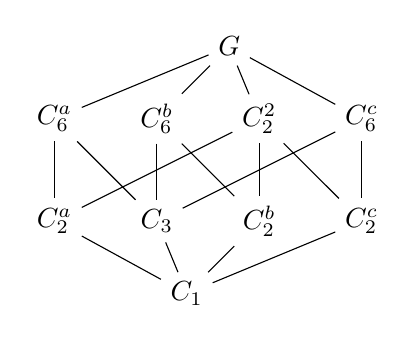
\begin{tikzpicture}[node distance=1.3cm]
        \node(G)[midway]{$G$};
        \node(C6b)[below left of =G]{$C_6^{b}$}; \node(C6a)[left of=C6b]{$C_6^{a}$};  
        \node(C22)[right of=C6b]{$C_2^{2}$};    \node(C6c)[right of=C22]{$C_6^{c}$};
        \node(C2a)[below of=C6a]{$C_2^{a}$};    \node(C3)[below of=C6b]{$C_3$};
        \node(C2b)[below of=C22]{$C_2^{b}$};    \node(C2c)[below of=C6c]{$C_2^{c}$};
        \node(C1)[below left of=C2b]{$C_1$};
        \draw(G)--(C6a);    \draw(G)--(C6b);    \draw(G)--(C6c);    \draw(G)--(C22);
        \draw(C6a)--(C2a);  \draw(C6a)--(C3);
        \draw(C6b)--(C2b);  \draw(C6b)--(C3);
        \draw(C6c)--(C2c);  \draw(C6c)--(C3);
        \draw(C22)--(C2a);  \draw(C22)--(C2b);  \draw(C22)--(C2c);
        \draw(C2a)--(C1);   \draw(C2b)--(C1);   \draw(C2c)--(C1);   \draw(C3)--(C1); 
    \end{tikzpicture}
    \end{figure}
    %There is a Brauer relation coming from the $C_2 \times C_2$-quotient, given by $$\Psi = C_3 - C_6^a - C_6^b - C_6^c + 2G.$$ 
    
    Consider an order $6$ character $\rho_a$ of $G$ with $C_2^{a}$ in its kernel. This has $\bQ(\rho_a) = \bQ(\zeta_6) = \bQ(\sqrt{-3})$. Let $\tau$ generate $\Gal(\bQ(\rho_a) / \bQ)$. One has
    \begin{equation}\label{ex1-rel}\tag{\textdagger}
    \Ind_{C_2^{a}}^G \trivial  \ominus \Ind_{C_6^{a}}^G \trivial \ominus \Ind_{C_2^{2}}^G \trivial \oplus \Ind_G^G \trivial \simeq \rho_a \oplus \rho_a^{\tau} .
    \end{equation}
    Let $E / \bQ$ be a semistable elliptic curve. To apply Theorem \ref{thm_positive_rank}, we need to compute
    \begin{equation}\label{ex1}\tag{*} 
        \frac{C_{E / F^{C_2^a}} C_{E / \bQ} }{C_{E / F^{C_6^a}} C_{E / F^{C_2^2}}} = 
        \frac{C_{E / L} C_{E / \bQ}}{C_{E / L^{C_3}} C_{E / L^{C_2}}}
    \end{equation} 
    where $L = F^{C_2^a}$ has $\Gal(L / \bQ) = C_6$, and check whether it is a norm from $\bQ(\sqrt{-3})$. This is a product of local Tamagawa numbers, as the minimal differential terms are $1$ when $E / \bQ$ is semistable (Lemma \ref{lem_Dterms}(i)). 
    
    One needs to compute these locally for each $p \in \bQ$. If $E / \bQ_p$ has good reduction, then the Tamagawa numbers at all places above $p$ in the subfields of $L$ are $1$. Suppose that $E / \bQ_p$ has split multiplicative reduction at $p$. Let $n = v_p(\Delta_E)$. For $H \leq G$, the Tamagawa number at a prime $\fp$ above $p$ in $L^H$ is given by $c_{\fp}(E / L^H) = e_{\fp / p} n$, where $e_{\fp \mid p}$ is the ramification degree. Thus the computation of Tamagawa numbers depends on the choice of decomposition group $D_p \leq C_6$ (to count the number of primes above $p$ in a given subfield) and the choice of inertia group $I_p \leq C_6$ (to compute the ramification indices). The following table describes the product of Tamagawa numbers at places above $p$ in our expression, for varying $D_p$ and $I_p$. We let $C_{\fp \mid p}(E / L^H) = \prod_{\fp \mid p}c_{\fp}(E / L^H_{\fp})$ for $H \leq \Gal(L / \bQ)$, and write $C_p = c_p(E / \bQ)C_{\fp \mid p}(E / L) \big/ C_{\fp \mid p}(E / L^{C_3})C_{\fp \mid p}(E / L^{C_2})$. 
    \[
    \begin{array}{c c c c c c c}
        D_p & I_p & c_p(E / \bQ) & C_{\fp \mid p}(E / L^{C_3}) & C_{\fp \mid p}(E / L^{C_2}) & C_{\fp \mid p}(E / L) & C_p\\ 
        \hline
        C_1 & C_1 & n & n^2 & n^3 & n^6 & \square\\
        C_2 & C_1 & n & n & n^3 & n^3 & \square\\
        C_3 & C_1 & n & n^2 & n & n^2 & \square \\
        C_6 & C_1 & n & n & n & n & \square \\
        C_2 & C_2 & n & 2n & n^3 & (2n)^3 & \square \\
        C_6 & C_2 & n & 2n & n & 2n & \square \\
        C_3 & C_3 & n & n^2 & 3n & (3n)^2 & 3\cdot\square \\
        C_6 & C_3 & n & n & 3n & 3n & \square\\
        C_6 & C_6 & n & 2n & 3n & 6n & \square
    \end{array}
    \]

    In all cases we see that $C_p$, the contribution of Tamagawa numbers above $p$, is a norm form $\bQ(\sqrt{-3})$. It is not too hard to check that this is also the case when $E / \bQ_p$ has non-split multiplicative reduction. Therefore the expression in \eqref{ex1} is always a norm from $\bQ(\rho_a)$. This is an example of a more general phenomenon; for cyclic groups and semistable elliptic curves we always get a norm. This follows from  Theorem \ref{thm_consistent_cyclic}, which is proven in \S\ref{sec-cyclic}.
    %and $F / \bQ$ an abelian extension with $G = \Gal(F / \bQ)$. We claim that $C(\Theta) \in \fieldnorm{\rho_a}$, for all such $E$. Since each subgroup in $\Theta$ contains $C_2^{a}$, we have that $C(\Theta)$ equals $C(\Theta / C_2^{a})$ where $\Theta / C_2^{a} \in \B(G / C_2^{a}) = \B(C_6)$.  Now $\Theta / C_2^{a}$ is a $\chi_6$-relation, where $\chi_6 = \rho_a^{C_2^a}$ is a faithful order $6$ character of $C_6$, with $\bQ(\chi_6) = \bQ(\rho_a)$. But for cyclic groups we always get norm relations; by Theorem \ref{thm_consistent_cyclic}, $C(\Theta / C_2^{a}) \in \fieldnorm{\rho_a}$.

    But! Observe that{\footnote{this is called a Brauer relation, see Definition \ref{def-brauer}}} 
    \[ \Ind_{C_3}^G \trivial \ominus \Ind_{C_6^a}^G \trivial \ominus \Ind_{C_6^b}^G \trivial \ominus \Ind_{C_6^c}^G \trivial \oplus (\Ind_G^G \trivial)^{\oplus 2} = 0 \]
    as a virtual permutation representation. We can append this to the left hand side of \eqref{ex1-rel}. Then Theorem \ref{thm_positive_rank} asks us to compute 
    \begin{equation}\label{ex1-rel2}\tag{**}
    \left(\frac{C_{E / F^{C_2^a}} C_{E / \bQ} }{C_{E / F^{C_6^a}} C_{E / F^{C_2^2}}}\right) \cdot \left( \frac{C_{E / F^{C_3}} C_{E / \bQ}^2}{C_{E / F^{C_6^a}}C_{E / F^{C_6^b}}  C_{E / F^{C_6^c}} } \right). 
    \end{equation}
    
    We can find instances where the second factor is not a norm from $\bQ(\sqrt{-3})$. Indeed suppose $E / \bQ$ has split multiplicative reduction at a prime $p$ with $D_p = G$, $I_p = C_6^b$ (assuming tamely ramified, one can take a prime $p$ such that $6 \mid p^2 - 1$, e.g. $p = 5$). Let $v_p(\Delta_E) = n$. Then there is only one prime above $p$ in each subfield. Suppose $E$ has good reduction at all other primes (or multiplicative reduction at primes that are totally split in $F / \bQ$ would also be fine).
     Then our expression \eqref{ex1-rel2} is equal to
     \[ \frac{(6n)(n)}{(2n) (3n)} \cdot \frac{(2n)(n)^2}{(2n)(n)(2n)} = \frac{1}{2} \cdot \square,\] 
     but $\frac{1}{2}$ is not a norm in $\bQ(\sqrt{-3})$. Hence one must have $\rk E / F > 0$. 
\end{example}

\begin{example}[Dihedral]
    Let $q_1, q_2$ be odd primes. Consider $G = D_{2 q_1 q_2}$ the dihedral group of order $2 q_1 q_2$. 
    Let $\rho$, $\tau_1$, $\tau_2$ be two-dimensional irreducible representations of $G$ corresponding to rotating a $(q_1 q_2)$-gon by $2 \pi / q_1 q_2$, $2 \pi / q_1$, $2 \pi q_2$ respectively. The Galois conjugates of these representations, as well as the trivial $\trivial$ and sign $\epsilon$, yield all the irreducible representations of $G$. One has
    \begin{table}[H]
        \centering
    \begin{tabular}{l}
        $\Ind_{C_2}^G \trivial \simeq \trivial \oplus \repnorm{\tau_1} \oplus \repnorm{\tau_2} \oplus \repnorm{\rho},$ \\
        $\Ind_{D_{2 q_1}}^G \trivial \simeq \trivial \oplus \repnorm{\tau_2}$,\\
        $\Ind_{D_{2 q_2}}^G \trivial \simeq \trivial \oplus \repnorm{\tau_1}$.
    \end{tabular}
\end{table}
% There is an irreducible representation $\rho$ of $G$, obtained by inducing a linear order $q_1 q_2$ faithful representation from $C_{q_1 q_2}$. Thus $\rho$ is of degree $2$ and $\bQ(\rho) = \bQ(\zeta_{q_1 q_2})^{C_2}$. Then $\rho$ has $\frac{(q_1 - 1)(q_2 - 1)}{2}$ Galois conjugates, and so $\repnorm{\rho}$ is of dimension $2 \cdot \frac{(q_1 - 1)(q_2 - 1)}{2}$. 
Thus there is a $\rho$-relation $$\Theta = C_2 - D_{2 q_1} - D_{2 q_2} + G, \qquad \bC[G / \Theta] \simeq \repnorm{\rho}.$$ 

    Suppose that $E / \bQ$ is semistable. Recall that $C(\Theta) = \prod_p C_{\fp \mid p}(\Theta)$. Suppose that $E / \bQ_p$ has split multiplicative reduction, with $n = v_p(\Delta_E)$. Then by Proposition \ref{prop_local_fns}, $C_{\fp \mid p} = (D_p, I_p, en)$. Corollary \ref{cor-odd-decomp} implies that $C_{\fp \mid p}(\Theta)$ is a norm from the quadratic subfields of $\bQ(\rho)$ whenever $|D_p|$ is odd. In fact, ranging over all possible $D_p$ and $I_p$, a case by case analysis yields that $C_{\fp \mid p}(\Theta)$ is non-square only when the decomposition group is $D_{2 q_1}$ or $D_{2 q_2}$ (and $I_p$ is non-trivial). 

    For example, let $p$ have decomposition group $D_{2 q_1}$ and inertia group $C_{q_1}$. We use Exercise \ref{ex-counting} to compute $(D_p, I_p, en)$ on each subgroup in $\Theta$:
        \begin{itemize}[--]
            \setlength\itemsep{0em}
            \item The action of $D_{2 q_1}$ on $C_2 \backslash G$ yields $1$ orbit of size $C_{q_1}$ (the orbit of the identity) and $\frac{q_2 - 1}{2}$ orbits of size $2q_1$ (coming from $C_2$ acting faithfully on $C_{q_2}$). The size of the inertia sub-orbits is $q_1$. Hence $C_{\fp \mid p}(C_2) = (q_1 n)^{1 + \frac{q_2 - 1}{2}}$.
            \item The action of $D_{2 q_1}$ on $D_{2 q_1} \backslash G$ yields the same number of orbits as above, but now the action of $C_{q_1} \leq D_{2 q_1}$ is trivial and the size of the inertia sub-orbits are all $1$, so that $C_{\fp \mid p}(D_{2 q_1}) = n^{1 + \frac{q_2 - 1}{2}}$.
            \item The action of $D_{2 q_1}$ on $D_{2 q_2} \backslash G$ yields one orbit of size $q_1$, with the inertia sub-orbit also of size $q_1$, hence $C_{\fp \mid p}(D_{2 q_2}) = q_1 n$.
        \end{itemize}
    In total,
    \[ C_{\fp \mid p}(\Theta) = \frac{(q_1 n )^{1 + \frac{q_2 - 1}{2}} (n)}{(n)^{1 + \frac{q_2 - 1}{2}} (q_1 n)} = q_1^{\frac{q_2 - 1}{2}} .\] 
    By symmetry, taking the decomposition group to be $D_{2 q_2}$ and inertia group $C_{q_2}$, one has 
     $C_{\fp \mid p}(\Theta) = q_2^{\frac{q_1 - 1}{2}}$.

    So let $E / \bQ$ have split multiplicative reduction at $p$ with decomposition group $D_{2 q_1}$ and inertia group $I_p = C_{q_1}$, and good reduction at all other primes. Further suppose that $q_1, q_2 \equiv 3 \pmod 4$ and that $\legendre{q_1}{q_2} = -1$. Then $\bQ(\sqrt{q_1 q_2}) \subset \bQ(\rho)$ but $C_{\fp \mid p}(\Theta) \not\in N_{\bQ(\sqrt{q_1 q_2}) / \bQ}(\bQ(\sqrt{q_1 q_2})^{\times})$. Indeed, one has $C_{\fp \mid p}(\Theta) \equiv q_1 \mod (\bQ^{\times})^2$, but $q_1$ is not the norm of an element of $\bQ(\sqrt{q_1 q_2})$, since $z^2 q_1 = x^2 - q_1q_2 y^2$ for $x,y,z \in \bZ$ implies $q_1 = \square \pmod {q_2}$, a contradiction. Thus $\rk E / F > 0$.

    This rank growth is predicted by root number computations also, however. Assume that $F / \bQ$ is totally real. Then $w(E / F^H) = (-1)^{[F^H \colon \bQ] + | H \backslash G / D_p|}$ by Proposition \ref{compute-root}. Thus
    \begin{itemize}[--]
        \setlength\itemsep{0em}
        \item $w(E / \bQ) = (-1)^2 = 1$,
        \item $w(E / F^{C_2}) = (-1)^{q_1 q_2} (-1)^{1 + \frac{q_2 - 1}{2}} = (-1)^{\frac{q_2 - 1}{2}}$,
        \item $w(E / F^{D_{2 q_1}}) = (-1)^{q_2}(-1)^{1 + \frac{q_2 - 1}{2}} = (-1)^{\frac{q_2 - 1}{2}},$
        \item $w(E / F^{D_{2 q_2}}) = (-1)^{q_1}(-1) = 1$. 
    \end{itemize}
    Therefore we must have $\rk E / F^{C_2}$, $\rk E / F^{D_{2q_1}} > 0$, so $\rk E / F > 0$. 
    Using the properties in Proposition \ref{compute-root-twist}, the computations of the root numbers for the subfields implies that 
    \[ w\left(E / \bQ, \repnorm{\tau_1}\right) = 1, \quad w\left(E / \bQ, \repnorm{\tau_2}\right) = -1, \quad w\left(E / \bQ, \repnorm{\rho}\right) = 1, \]
  and in particular there is an irreducible self-dual Artin rep $\tau'$ with $w(E / \bQ, \tau') = -1$ (some irreducible consistent of $\repnorm{\tau_2}$). In particular the parity conjecture for twists implies that $\left\langle \repnorm{\tau'}, E(F)_{\bC} \right\rangle > 0$. 
    
  
  {\color{red} maybe I could add how this suggests we throw in a $q_1$ for the regulators and then everything is fine }
\end{example}

\begin{example}[Additive reduction example]



\end{example}


\newpage
\section{Consistency cases with BSD}
As we discussed in the previous section, our motivation is to use Theorem \ref*{thm_positive_rank} to predict points of infinite order for families of elliptic curves. However, in this section we prove that in several cases the theorem will never make such a prediction. In other words, in such cases, the product 
$$\frac{\prod_i C_{E/F_i}}{\prod_j C_{E/F_j'}}$$ 
is always a norm for every subfield $\QQ(\sqrt{D})\subseteq\QQ(\rho)$.

\subsection{Cyclic Extensions}
In this subsection we prove the following. 
\begin{thm}\label{thm_consistent_cyclic}
    Let $E/\QQ$ be a semistable elliptic curve and let $F$ be a finite cyclic Galois extension $\QQ$ so that $\Gal(F/\QQ)=C_d$ for some $d\geq 2$. Let $\chi$ be a faithful character of $C_d$ (so that $\QQ(\chi)=\QQ(\zeta_d)$), and let $F_i,F'_j\subseteq F$ be such that
    $$\bigoplus_{\mathfrak{g}\in\Gal(\QQ(\zeta_d)/\QQ)}\chi^{\mathfrak{g}}=\bigoplus_i\Ind_{F_i/\QQ}\mathds{1}\ominus\bigoplus_j\Ind_{F'_j/\QQ}\mathds{1}.$$
    Then for any $\QQ(\sqrt{D})\subseteq\QQ(\zeta_d)$,
    $$\frac{\prod_i C_{E/F_i}}{\prod_j C_{E/F_j'}}$$
    is a norm of $\QQ(\sqrt{D})$. Moreover, the contribution is always the square of rational number unless $d=2^n, p^n,2p^n$ for some odd prime $p$.
\end{thm}

The first step in proving Theorem \ref*{thm_consistent_cyclic} is to show that the fields $F_i, F'_j$ exist, and to give a precise description. Recall that for each $k\mid d$ the cyclic group $C_d$ has one unique subgroup of order $k$, which is of course also cyclic. Therefore, for each $k\mid d$, there is one unique subfield $L_k$ of $F$ of degree $k$ over $\QQ$ which is also cyclic. Under the Galois correspondence, this field corresponds to the subgroup $H_k=\Gal(F/L_k)=C_{d/k}$.

To give the required description, we recall that the Möbius function $\mu$ is the function supported on the square-free integers, and $\mu(n)=(-1)^s$ whenever $n$ is square free and $s$ is the number of prime factors of $n$.

\begin{lemma}\label{lem_cyclic_decomp}
    Let $E/\QQ$, $F$ and $\chi$ be as in Theorem \ref*{thm_consistent_cyclic}. Writing characters of $C_d$ additively, we have that
    \begin{equation}\label{eqn_cyclic_relation}
        \sum_{\mathfrak{g}\in\Gal(\QQ(\zeta_d)/\QQ)}\chi^{\mathfrak{g}}=\sum_{k\mid d}\mu(d/k)\Ind_{L_k/\QQ}\mathds{1}.
    \end{equation}
    Furthermore, such an expression is unique.
\end{lemma}

\begin{rem}\label{rem_radical}
    This lemma has an important consequence. Given an integer $d\geq2$, let $\rad(d)=\prod_{p\mid d}p$ be the radical of $d$, and let $K=L_{d/\rad(d)}$ be the unique subfield of $F$ such that $[F:K]=\rad(d)$. For $k\mid d$, $\mu(d/k)\neq 0$ precisely when $[K:\QQ]=\frac{d}{\rad(d)}\mid k$ and therefore the fields appearing in the right hand side of \eqref{eqn_cyclic_relation} are the fields $L_k$ satisfying $K\subseteq L_k\subseteq F$. 
\end{rem}

Following this observation, we will compute the product of the local factors locally for each finite place $\pp$ of $K$ and the places above it in the other fields $L_k\supseteq K$. To that objective, the following notation will be useful.

\begin{notation}\label{not_local_contr}
    Let $E/\QQ$, $F$ and $\chi$ be as in Theorem \ref*{thm_consistent_cyclic}, and let $L_k$ and $K$ be as in Remark \ref*{rem_radical}. For a finite place $\pp$ of $K$, we write
    $$\contr_\chi(\pp)=\prod_{\frac{d}{\rad(d)}\mid k\mid d}C_{\mathfrak{P}\mid\pp}(L_k/K)^{\mu(d/k)}=\prod_{k\mid d}C_{\mathfrak{P}\mid\pp}(L_k/K)^{\mu(d/k)}$$ 
    where the terms in the product are defined as in Notation \ref*{not_contr}. 
\end{notation}

An immediate consequence of the above definition is the fact that 
\begin{equation}\label{eqn_local_contr}
    \prod_{k\mid d}(C_{E/L_k})^{\mu(d/k)}=\prod_\pp\contr_\chi(\pp),
\end{equation}

and therefore we can calculate the product of local terms \textbf{locally}, one prime $\pp$ at a time.

We divide the proof of Theorem \ref*{thm_consistent_cyclic} into two cases: odd and even cyclic extensions. The main idea in both cases is to simplify the general case into smaller cases where we can directly compute $\contr_\chi(\pp)$ for each finite place $\pp$ of $K$. We note that if $E$ has good reduction over $\pp$, then $\contr_\chi(\pp)=1$ and therefore we focus our attention to bad semistable reduction. 

\subsection*{Odd Cyclic Extensions} \label{case_Cp}

For the first case, we assume that $d$ is odd. Following the observation in Remark \ref*{rem_radical}, we need to calculate $\contr_\chi(\pp)$ for each finite place $\pp$ of $K$. To that objective, we first calculate them for ``small'' cases and then we use them for the general case. The following lemmas build on this idea.

\begin{lemma}\label{lem_Cp}
    Let $p$ be a rational prime, $F/K$ a Galois extension of number fields such that $\Gal(F/K)=C_p$ and $E/\QQ$ an elliptic curve. Then 
    $$\frac{C_{E/F}}{C_{E/K}}$$
    is a rational square up factors of $p$.
\end{lemma}

\begin{proof}
    Fix some prime $\pp$ in $K$. Since the extension $L/K$ is cyclic, the splitting behaviour in $L$ is determined by the ramification index $e_\pp$ and the residual degree $f_\pp$. Since $\contr_\chi(\pp)=1$ if $E$ has good reduction at $\pp$ and $E$ is assumed to be semistable, we assume that $E$ has split or non-split multiplicative reduction. The following table records the contribution of $\pp$ dependinng on $e_\pp$ and $f_\pp$, and the entries for split and non-split multiplicative reduction of type $\mathrm{I}_n$ are separated by a ``;''.
    \begin{table}[h!]
        \centering
        \begin{tabular}{|l|l|l|l|l|}
        \hline
        $e_\pp$ & $f_\pp$  & $C_{\mathfrak{P}\mid \pp}(K/K)$ & $C_{\mathfrak{P}\mid \pp}(F/K)$  & $\contr_\chi(\pp)$ \\ \hline
        $1$ & $1$ & $n;\tilde{n}$ & $n^p;\tilde{n}^p$ & $\square$ \\ \hline
        $p$ & $1$ & $n;\tilde{n}$ & $pn;\tilde{n}$ & $p\square;\square$ \\ \hline
        $1$ & $p$ & $n;\tilde{n}$ & $n;\tilde{n}$ & $\square$ \\ \hline
        \end{tabular}
    \end{table}
    The proof follows immediately from \eqref{eqn_local_contr}.
\end{proof}

Next, we prove an analogous result for $C_{pq}$ extensions, where $p$ and $q$ are odd rational primes.

\begin{lemma}\label{lem_Cpq}
    Let $p,q$ be distinct, odd rational primes and let $F/K$ be a Galois extension of number fields such that $\Gal(F/K)=C_{pq}$. Let $E/\QQ$ be an elliptic curve and let $L_k$ be the fields as above. Then
    $$\frac{C_{E/F}C_{E/K}}{C_{E/L_p}C_{E/L_q}}$$
    is always a rational square.
\end{lemma}

\begin{proof}
    The idea of the proof is identical to Lemma \ref*{lem_Cp} since in a $C_{pq}$ extension $L/K$ the splitting behaviour of a prime $\pp$ of $K$ in $L$ and all the intermediate fields is determined by $e_\pp$ and $f_\pp$. The following table records the contribution of $\pp$ depending on these values, and again the entries for split and non-split multiplicative reduction of type $\mathrm{I}_n$ are separated by ``;''.

    \begin{table}[!ht]
        \centering
        \begin{tabular}{|l|l|l|l|l|l|l|}
        \hline
        $e_\pp$ & $f_\pp$  & $C_{\mathfrak{P}\mid \pp}(K)$ & $C_{\mathfrak{P}\mid \pp}(L_p)$ & $C_{\mathfrak{P}\mid \pp}(L_q)$ & $C_{\mathfrak{P}\mid \pp}(F)$ & $\contr_\chi(\pp)$ \\ \hline
        $1$ & $1$ & $n;\tilde{n}$ & $n^p;\tilde{n}^p$ & $n^q;\tilde{n}^q$ & $n^{pq};\tilde{n}^{pq}$ & $\square$ \\ \hline
        $1$ & $p$ & $n;\tilde{n}$ & $n;\tilde{n}$ & $n^q;\tilde{n}^q$ & $n^q;\tilde{n}^q$ & $\square$ \\ \hline
        $1$ & $q$ & $n;\tilde{n}$ & $n^p;\tilde{n}^p$ & $n;\tilde{n}$ & $n^p;\tilde{n}^p$ & $\square$ \\ \hline
        $1$ & $pq$ & $n;\tilde{n}$ & $n;\tilde{n}$ & $n;\tilde{n}$ & $n;\tilde{n}$ & $\square$ \\ \hline
        $p$ & $1$ & $n;\tilde{n}$ & $pn;\tilde{n}$ & $n^q;\tilde{n}^q$ & $p^qn^q;\tilde{n}^q$ & $\square$ \\ \hline
        $p$ & $q$ & $n;\tilde{n}$ & $pn;\tilde{n}$ & $n;\tilde{n}$ & $pn;\tilde{n}$ & $\square$ \\ \hline
        $q$ & $1$ & $n;\tilde{n}$ & $n^p;\tilde{n}^p$ & $qn;\tilde{n}$ & $q^pn^p;\tilde{n}^p$ & $\square$ \\ \hline
        $q$ & $p$ & $n;\tilde{n}$ & $n;\tilde{n}$ & $qn;\tilde{n}$ & $qn;\tilde{n}$ & $\square$ \\ \hline
        $pq$ & $1$ & $n;\tilde{n}$ & $pn;\tilde{n}$ & $qn;\tilde{n}$ & $pqn;\tilde{n}$ & $\square$ \\ \hline
        \end{tabular}
    \end{table}
Again, the result follows immediately from the table and \eqref{eqn_local_contr}.
    \begin{figure}[!ht]
        \centering
        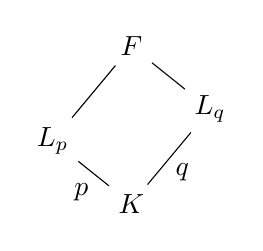
\begin{tikzpicture}

            \node (Q1) at (0,0) {$K$};
            \node (Q2) at (1,1.2) {$L_q$};
            \node (Q3) at (0,2) {$F$};
            \node (Q4) at (-1,0.8) {$L_p$};
        
            \draw (Q1)--(Q2) node [pos=0.8, below,inner sep=0.25cm] {$q$};
            \draw (Q1)--(Q4) node [pos=0.9, below,inner sep=0.25cm] {$p$};
            \draw (Q3)--(Q4);
            \draw (Q2)--(Q3);
        
        \end{tikzpicture}
        \caption[short]{Subfields of a $C_{pq}$-extension}
    \end{figure}
\end{proof}

We are finally ready to prove the main result of this section, from which Theorem \ref*{thm_consistent_cyclic} will follow. 

\begin{lemma}\label{lem_Cd_odd}
    Let $d$ be a composite, odd squarefree integer and let $F/K$ be a Galois extension of number fields such that $\Gal(F/K)=C_{d}$. Let $E/\QQ$ be an elliptic curve and let $L_k$ be the fields as above. Then
    $$\prod_{k\mid d}(C_{E/L_k})^{\mu(d/k)}$$
    is always a rational square.
\end{lemma}

\begin{proof}
    Let $n$ be the number of distinct prime numbers dividing $d$, so that $d=p_1\ldots p_n$ for some distinct odd primes $p_i$. We prove this result by induction. The base case for $n=2$ is the content of Lemma \ref*{lem_Cpq}. Assume that the result holds for squarefree integers with $n-1$ prime factors and consider the two sets of fields
    $$\mathcal{A}=\{L_k:p_n\nmid k\}\quad\text{and}\quad\mathcal{B}=\{L_k:p_n\mid k\},$$
    which are clearly a partition of all intermediate fields of $F/K$. Furthermore, the fields in $\mathcal{A}$ are precisely the intermediate fields of $K$ and $L_{d/p_n}$, while the fields in $\mathcal{B}$ are the intermediate fields of $L_{p_n}$ and $F$. However, since $\Gal(L_{d/p_n}/K)=\Gal(F/L_{p_n})=C_{d/p_n}$, it follows from the inductive hypothesis applied to the fields of $\mathcal{A}$ and $\mathcal{B}$ respectively that
    $$\prod_{k\mid \frac{d}{p_n}}(C_{E/L_k})^{\mu\left(\frac{d}{kp_n}\right)}\quad\text{and}\quad\prod_{p_n\mid k\mid d}(C_{E/L_{k}})^{\mu\left(d/k\right)}$$
    are both rational squares. By the natural decomposition
    $$\prod_{k\mid d}(C_{E/L_k})^{\mu(d/K)}=\prod_{k\mid \frac{d}{p_n}}(C_{E/L_k})^{\mu\left(d/k\right)}\prod_{p_n\mid k\mid d}(C_{E/L_{k}})^{\mu\left(d/k\right)}=\left(\prod_{k\mid \frac{d}{p_n}}(C_{E/L_k})^{\mu\left(\frac{d}{kp_n}\right)}\right)^{-1}\prod_{p_n\mid k\mid d}(C_{E/L_{k}})^{\mu\left(d/k\right)},$$
    it follows that the left hand side is also a rational square, as desired.
    \begin{figure}[!ht]
        \centering
        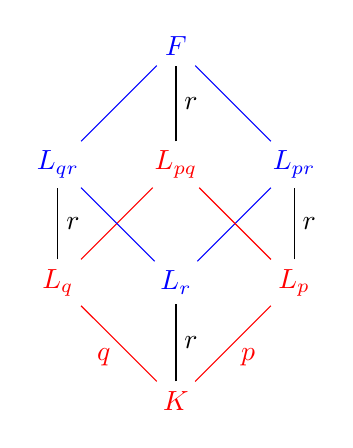
\begin{tikzpicture}

            \node [red] (Q1) at (0,0) {$K$};
            \node [red] (Q2) at (-1.5,1.5) {$L_q$};
            \node [blue] (Q3) at (0,1.5) {$L_r$};
            \node [red] (Q4) at (1.5,1.5) {$L_p$};
            \node [blue] (Q5) at (-1.5,3) {$L_{qr}$};
            \node [red] (Q6) at (0,3) {$L_{pq}$};
            \node [blue] (Q7) at (1.5,3) {$L_{pr}$};
            \node [blue] (Q8) at (0,4.5) {$F$};

            \draw [red] (Q1)--(Q2) node [pos=0.7, below,inner sep=0.25cm] {$q$};
            \draw [red] (Q1)--(Q4) node [pos=0.7, below,inner sep=0.25cm] {$p$};
            \draw (Q1)--(Q3) node [pos=0.5, right,inner sep=0.1cm] {$r$};
            \draw (Q2)--(Q5) node [pos=0.5, right,inner sep=0.1cm] {$r$};
            \draw (Q2)--(Q6) [red];
            \draw (Q3)--(Q5) [blue];
            \draw (Q3)--(Q7) [blue];
            \draw (Q4)--(Q6) [red];
            \draw (Q4)--(Q7) node [pos=0.5, right,inner sep=0.1cm] {$r$};
            \draw (Q5)--(Q8) [blue];
            \draw (Q6)--(Q8) node [pos=0.5, right,inner sep=0.1cm] {$r$};
            \draw (Q7)--(Q8) [blue];
        
        \end{tikzpicture}
        \caption[short]{Partition of $n=3$ into $n=2$. Red fields are in $\mathcal{A}$ while blue fields are in $\mathcal{B}$.}
    \end{figure}
\end{proof}

We are now ready to prove Theorem \ref*{thm_consistent_cyclic} for odd $d$.

\begin{proof}[Theorem \ref*{thm_consistent_cyclic} for odd $d$]
    The proof is divided into two cases depending on whether $d$ is the power of a prime or not. Suppose first that $d$ is not, so that $\rad(d)$ is a squarefree \textbf{composite} number. However, by Remark \ref*{rem_radical} and Lemma \ref*{lem_Cd_odd} we know that 
    $$\frac{\prod_i C_{E/F_i}}{\prod_j C_{E/F'_j}}$$
    is a rational square, and therefore it is the norm of an element for any quadratic extension of $\QQ$. 

    The case when $d=p^n$ for some odd prime $p$ and $n\geq1$ requires some more work. Lemma \ref*{lem_cyclic_decomp} and Lemma \ref*{lem_Cp} show that 
    $$\frac{\prod_i C_{E/F_i}}{\prod_j C_{E/F'_j}}=\frac{C_{E/F}}{C_{E/L_{p^{n-1}}}}$$
    is a rational square up to factors of $p$. Therefore, it suffices to show that $p$ is the norm of any quadratic subextension of $\QQ(\zeta_{p^n})$. Since $\Gal(\QQ(\zeta_{p^n})/\QQ)=(\ZZ/p^n\ZZ)$ is cyclic, $\QQ(\zeta_{p^n})$ has one unique quadratic subextension. Hence, it suffices to find the unique quadratic subextension of $\QQ(\zeta_p)$. A simple calculation shows that 
    $$\left(\sum_{a=0}^{p-1}\left(\frac{a}{p}\right)\zeta_p^a\right)^2=(-1)^{(p-1)/2}p,$$
    and therefore $\QQ(\sqrt{p^*})$ is the unique quadratic subextension of $\QQ(\zeta_p)$, where $p^*=(-1)^{(p-1)/2}p$. The fact that $p$ is a norm in this field is precisely the content of Corollary \ref*{p-norm}, and so the Theorem follows.
\end{proof}
 
\subsection*{Even Cyclic Extensions}
A bit more care is required to prove Theorem \ref*{thm_consistent_cyclic} for even $d$. This difficulty mainly lies in the case when $d$ is only divisible by one odd prime $p$. Likewise to the earlier case, we first prove some relevant results.

\begin{lemma}\label{lem_C2p}
    Let $p$ be an odd prime and let $F/K$ be a Galois extension of number fields such that $\Gal(F/K)=C_{2p}$ and let $L_k$ be the fields as above. Let $E/\QQ$ be an elliptic curve. Then
    $$\frac{C_{E/F}C_{E/K}}{C_{E/L_2}C_{E/L_p}}$$
    is a rational square up to factors of $p$.
\end{lemma}

\begin{proof}
    The proof is identical to the proof of Lemmas \ref*{lem_Cp} and \ref*{lem_Cpq} since the splitting behaviour of a prime $\pp$ in $K$ is again determined by $e_\pp$ and $f_\pp$. The following table records the contribution.

    \begin{table}[!ht]
        \centering
        \begin{tabular}{|l|l|l|l|l|l|l|}
        \hline
        $e_\pp$ & $f_\pp$  & $C_{\mathfrak{P}\mid \pp}(\QQ)$ & $C_{\mathfrak{P}\mid \pp}(L_p)$ & $C_{\mathfrak{P}\mid \pp}(L_2)$ & $C_{\mathfrak{P}\mid \pp}(F)$ & $\contr_\chi(\pp)$ \\ \hline
        $1$ & $1$ & $n;\tilde{n}$ & $n^p;\tilde{n}^p$ & $n^2;\tilde{n}^2$ & $n^{2p};\tilde{n}^{2p}$ & $\square$ \\ \hline
        $1$ & $p$ & $n;\tilde{n}$ & $n;\tilde{n}$ & $n^2;\tilde{n}^2$ & $n^2;\tilde{n}^2$ & $\square$ \\ \hline
        $1$ & $2$ & $n;\tilde{n}$ & $n^p;\tilde{n}^p$ & $n;n$ & $n^p;n^p$ & $\square$ \\ \hline
        $1$ & $2p$ & $n;\tilde{n}$ & $n;\tilde{n}$ & $n;n$ & $n;n$ & $\square$ \\ \hline
        $p$ & $1$ & $n;\tilde{n}$ & $pn;\tilde{n}$ & $n^2;\tilde{n}^2$ & $p^2n^2;\tilde{n}^2$ & $p\square;\square$ \\ \hline
        $p$ & $2$ & $n;\tilde{n}$ & $pn;\tilde{n}$ & $n;n$ & $pn;n$ & $\square$ \\ \hline
        $2$ & $1$ & $n;\tilde{n}$ & $n^p;\tilde{n}^p$ & $2n;1$ & $2^pn^p;1^p$ & $\square$ \\ \hline
        $2$ & $p$ & $n;\tilde{n}$ & $n;\tilde{n}$ & $2n;1$ & $2n;1$ & $\square$ \\ \hline
        $2p$ & $1$ & $n;\tilde{n}$ & $pn;\tilde{n}$ & $2n;1$ & $2pn;1$ & $\square$ \\ \hline
        \end{tabular}
    \end{table}
    The result follows again from \eqref{eqn_local_contr}.

\end{proof}

However, as soon as $d$ is divisible by $4$, the product of local factors is a rational square even if the individual contributions might not be, as the next lemma suggests. 

\begin{lemma}\label{lem_C4p}
    Let $p$ be an odd prime and let $F/K$ be a Galois extension of number fields such that $\Gal(F/K)=C_{4p}$ and let $L_k$ be the fields as above. Let $E/\QQ$ be an elliptic curve. Then
    $$\frac{C_{E/F}C_{E/L_2}}{C_{E/L_4}C_{E/L_{2p}}}$$
    is a rational square.
\end{lemma}

\begin{proof}
    All fields appearing in the product are intermediate fields of $L_2$ and $F$, and $\Gal(F/L_2)=C_{2p}$. Lemma \ref*{lem_C2p} shows that given some prime $\pp$ in $L_2$, $\contr_\chi(\pp)$ is a square unless $e_\pp=p$ and $f_\pp=1$. That is, $\pp$ ramifies in $L_{2p}/L_2$ and is split in $L_4/L_2$. Now consider $\bar\pp=\pp\cap\mathcal{O}_K$. Since $\pp$ splits in $L_4$, this forces $\bar{\pp}$ to split as well in $L_2/K$. Hence, $\bar{\pp}=\pp\pp'$ for two \textbf{distinct} primes in $K$ that have the same splitting behaviour and therefore $\contr_\chi(\pp)\contr_\chi(\pp')$ is a rational square, as desired.

    \begin{figure}[!ht]
        \centering
        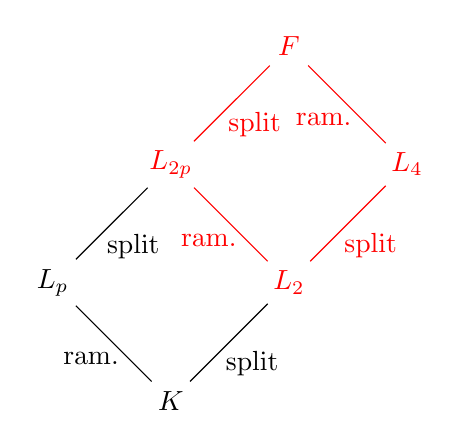
\begin{tikzpicture}

            \node (Q1) at (0,0) {$K$};
            \node (Q2) at (-1.5,1.5) {$L_p$};
            \node [red] (Q3) at (3,3) {$L_4$};
            \node [red] (Q4) at (1.5,1.5) {$L_2$};
            \node [red] (Q5) at (1.5,4.5) {$F$};
            \node [red] (Q6) at (0,3) {$L_{2p}$};
            

            \draw (Q1)--(Q2) node [pos=0.8, below,inner sep=0.4cm] {ram.};
            \draw (Q1)--(Q4) node [pos=0.8, below,inner sep=0.4cm] {split};
            \draw (Q2)--(Q6) node [pos=0.8, below,inner sep=0.4cm] {split};
            \draw [red] (Q3)--(Q5) node [pos=0.8, below,inner sep=0.4cm] {ram.};
            \draw [red] (Q4)--(Q6) node [pos=0.8, below,inner sep=0.4cm] {ram.};
            \draw [red] (Q6)--(Q5) node [pos=0.8, below,inner sep=0.4cm] {split};
            \draw [red] (Q4)--(Q3) node [pos=0.8, below,inner sep=0.4cm] {split};
        \end{tikzpicture}
        \caption[short]{\centering Field diagram for a $C_{4p}$ extension, together with the splitting\\ behaviour of a prime $\pp$ in $L_2$ with $e_\pp=p$ and $f_\pp=1$ over $F$.}
    \end{figure}
\end{proof}

We are now ready to prove Theorem \ref*{thm_consistent_cyclic} for even $d$. We break down the proof into three cases:

\subsubsection*{Case 1: $d$ is not divisible by any odd prime, so $d=2^l$}
If $l=1$, then $\QQ(\zeta_2)=\QQ$, so there is nothing to prove, so assume that $l\geq2$. If $\Gal(F/\QQ)=C_{2^l}$, then 
$$\frac{\prod_i C_{E/F_i}}{\prod_j C_{E/F'_j}}=\frac{C_{E/F}}{C_{E/L_{2^{l-1}}}},$$
and by Lemma \ref*{lem_Cp}, we know that this is a rational square up to factors of $2$, so it suffices to show that $2$ is a norm of every quadratic subfield of $\QQ(\zeta_{2^l})$. A standard argument shows that $\Gal(\QQ(2^l)/\QQ)=(\ZZ/2^l\ZZ)^*=C_{2^{l-2}}\times C_2$ and therefore $\QQ(\zeta_{2^l})$ has $\QQ(i)$ as its unique quadratic subextension if $l=2$ and has three quadratic subextensions if $l\geq 3$. Note that $\zeta_8=(1+i)/\sqrt{2}$ and therefore $\QQ(\zeta_8)=\QQ(i,\sqrt{2})$. The three quadratic subextensions are therefore $\QQ(i), \QQ(\sqrt{2})$ and $\QQ(\sqrt{-2})$. Then the result follows from the fact that 
$$2=\Norm_{\QQ(i)}(1+i)=\Norm_{\QQ(\sqrt{-2})}(2)=\Norm_{\QQ(\sqrt{2})}(2+\sqrt{2}).$$

\subsubsection*{Case 1: $d$ is divisible by at least two odd primes}
Let $K=L_{d/\rad(d)}$ be as in Remark \ref*{rem_radical} such that $\Gal(F/K)=C_{\rad(d)}$ and all fields appearing in the product of local factors contain $K$. Then using the same idea as in Lemma \ref*{lem_Cd_odd}, let 
$$\mathcal{A}=\{L_k\supseteq K:2\nmid [L_k:K]\}\quad\text{and}\quad\mathcal{B}=\{L_k\supseteq K:2\mid [L_k:K]\}.$$
Then the fiels in $\mathcal{A}$ and $\mathcal{B}$ are the intermediate fields of (distinct!) $C_{\rad(d)/2}$ extensions. These are odd cyclic extensions, and therefore by Lemma \ref*{lem_Cd_odd} the contribution is a rational square and therefore the norm of any quadratic extension.

\subsubsection*{Case 3: $d$ is divisible by one odd prime}
In this case, write $d=2^lp^n$ and let $L_k$ be the fields as above. In this case, we note that 
$$\frac{\prod_i C_{E/F_i}}{\prod_j C_{E/F'_j}}=\frac{C_{E/F}C_{E/L_{d/2p}}}{C_{E/L_{d/2}}C_{E/L_{d/p}}}.$$
By Lemma \ref*{lem_Cp}, we know that this product is a square up to multiples of $p$. If $l=1$, then $\Gal(\QQ(\zeta_{2p^n})/\QQ)=(\ZZ/2p^n\ZZ)^*=(\ZZ/p^n\ZZ)^*$ is cyclic, and therefore the unique quadratic subfield is $\QQ(\sqrt{p^*})$, and we already know that $p$ is a norm of this field.

From Lemma \ref*{lem_C2p} that the contribution of $p$ comes from those primes $\pp$ in $L_{d/2p}$ such that they ramify in $L_{d/2}$ and they split in $L_{d/p}$. However, as in the proof of Lemma \ref*{lem_C4p}, the prime $\bar{\pp}=\pp\cap L_{d/4p}$ must also split in $L_{d/2p}$ so $\bar{\pp}=\pp\pp'$ for $\pp'\neq\pp$ in $L_{d/2p}$. Since $\pp$ and $\pp'$ have the same splitting behaviour, they give the same contribution. Hence, the product of local terms is in fact a rational square and therefore the norm of any quadratic extension.

This concludes the proof of Theorem \ref*{thm_consistent_cyclic}, and we have in addition shown that the contribution is always a square except when $d=2^n,p^n$ or $2p^n$, where $p$ is an odd rational prime.
\qed

\subsection{Abelian Extensions}

\subsection{Odd-Degree Extensions}

\newpage
\begin{appendices}
\section{Algebraic number theory background}
%\subsection{Decompositions of primes in field extensions}
\subsection{Class field theory and genus fields}

In this section we introduce the concept of a genus field, as well as properties that will be useful for us.

Let $K$ be a number field. The \textbf{ideal class group} $\Cl_K = I_K / P_K$ is the group of fractional ideals modulo principal fractional ideals.
For an ideal $\fp$, we let $[\fp]$ denote its class in $\Cl_K$.

The \textbf{extended ideal class group} is the group $\Cl_K^{+} = I_K / P_K^{+}$, where
$P_K^{+}$ denotes the subgroup of principal fractional ideals with totally positive generator, i.e. ideals $\alpha \cO_K$ where $\sigma(\alpha) > 0$ for all real embeddings $\sigma \colon K \emb \bR$.

Note that $\Cl_K^{+}$ is the ray class group for the modulus $\fm$ of $K$ consisting of the product of all real places. The corresponding ray class field is known as the \textbf{extended Hilbert class field}, which we'll denote as $H^{+}$. This is the maximal extension of $K$ that is unramified at all finite primes. Let $H$ be the usual Hilbert Class field of $K$. Then one has $H \subset H^{+}$. Moreover, the index can be described in terms of the structure of $K$:

\begin{thm}\cite[Chapter VI, Section 3, Theorem 3.1]{Janusz}
    Let $r$ be the number of real primes of $K$. Let $U_K$, $U_K^{+}$ the group of units and totally positive units of $K$ respectively, Then 
    \[ [H^{+} \colon H] = 2^r [U_K \colon U_K^{+}]^{-1} .\]
\end{thm}
Observe that if $K$ has no real places, then $H^{+} = H$. For quadratic fields, the index depends on the norm of a fundamental unit:

\begin{cor}
    Let $K = \bQ(\sqrt{D})$ with $D$ a square-free positive integer. Let $\epsilon$ be a fundamental unit of $K$. Then $[H^{+} \colon H] = 1$ or $2$, according as $N_{K / \bQ}\left(\epsilon\right) = -1$ or $1$. 
\end{cor}


Fix $K = \bQ(\sqrt{D})$ for $D$ a squarefree integer. The (extended) Hilbert class field of $K$ need not be abelian over $\bQ$ (note that it is Galois over $\bQ$ by uniqueness of the (extended) Hilbert class field). However it can be useful to consider the maximal subfield of $H$ that is abelian over $\bQ$. 

\begin{defn}
    For any abelian extension $K / \bQ$, the \textbf{genus field} of $K / \bQ$ is the largest abelian extension $L / \bQ$ contained in $H$. The \textbf{extended genus field } is the largest abelian extension $L^{+} / \bQ $ contained in $H^{+}$.
\end{defn}

Let $\sigma \in \Gal(H^{+} / \bQ)$ be such that $\sigma|_{K}$ generates $\Gal(K / \bQ)$. $L$ has the following properties:

\begin{thm}\cite[Ch. VI, $\S$3, Theorem 3.3]{Janusz}\label{janusz-3.3}
    Let $K = \bQ(\sqrt{D})$.
    \begin{enumerate}
        \item $\Gal(H / L)$ is isomorphic to the subgroup of $C_K$ generated by the ideal classes of the form $[\sigma(\fU)\fU^{-1}]$, $\fU \in I_K$. 
        \item $\Gal(H / L) \simeq (C_K)^2$. 
    \end{enumerate}
\end{thm}

\begin{proof}[Proof sketch of 1.]
    Let $G = \Gal(H / \bQ)$. Then $L = H^{[G, G]}$ is the fixed field of the commutator subgroup of $G$. The Artin map induces an isomorphism $\varphi \colon C_K \to C \subset G$ with $\varphi(C_K) \simeq C = \Gal(H / K)$. One shows that $\varphi([\sigma(\fU)\fU^{-1}]) \in [G, C]$ and conversely that every commutator element in $[G, G]$ can be expressed as $\varphi([\sigma(\fU)\fU^{-1}])$ for some $\fU \in I_K$. 
\end{proof}

Note that this says that every class $[\sigma(\fU) \fU^{-1}]$ is a square in $C_K$.
This allows us to deduce the following:

\begin{thm}\label{p-principal}
Let $p$ be a prime in $\bQ$. If the residue degree of $p$ in $L / \bQ$ is $1$, then $p$ is the norm of a principal fractional ideal in $K$. 
\end{thm} 

\begin{proof}
Let $\varphi \colon C_K \to \Gal(H / K)$ be the isomorphism induced by the Artin map. By Theorem \ref{janusz-3.3}, $\Gal(L / K) = \Cl_K / \left(\Cl_K\right)^2$ is abelian. Let $\fp$ be a prime of $K$ lying over $p$. Then $N_{K / \bQ}(\fp) = p$ and $\fp$ has residue degree $1$ in $L$. It follows that $\varphi([\fp])|_{L} = \Id$ so that $\varphi([\fp]) \in \Gal(H / L)$. Thus by Theorem \ref{janusz-3.3} there is a fractional ideal $\fU$ of $I_K$ such that 
$[\fp] = [\sigma(\fU)\fU^{-1}]$. Observe that $N_{K / \bQ}(\sigma(\fU)\fU^{-1}) = 1$. It follows that we can represent $[\fp]^n$ by a fractional ideal of norm $p$ for all $n$. Since $\Cl_K$ is finite, this implies there is a principal fractional ideal in $K$ of norm $p$. 
\end{proof}

Observe that $C_K / (C_K)^2$ is an abelian group of exponent $2$. The following theorem describes its order:

\begin{thm} 
Suppose the discriminant of $K / \bQ$ has $t$ prime divisors. Then $C_K / (C_K)^2$ has order $2^{t-1}$ if $D < 0$ or if $D > 0$ and a unit of $K$ has norm $-1$. Otherwise, if $D > 0$ and all units of $K$ have norm $1$, it has order $2^{t - 2}$.
\end{thm} 

Our introduction of the extended genus field $L^{+}$ is mostly because it is easier to describe than $L$ when $K = \bQ(\sqrt{D})$.

\begin{thm} 
Let the discriminant of $K$ be $\Delta$ and suppose $|\Delta| = p_1 p_2 \cdots p_t$ where $p_2, \ldots p_t$ are odd primes, and $p_1$ is either odd or a power of $2$. Then the extended genus field of $K$ is 
    \[ L^{+} = \bQ(\sqrt{D}, \sqrt{p_2^*}, \ldots \sqrt{p_t^*}) = K(\sqrt{p_2^*}, \ldots \sqrt{p_t^*}), \] 
where 
\[ \begin{cases}
    p_i^* = p_i & \mathrm{if }\ p_i \equiv 1 \pmod 4, \\
    p_i^* = -p_i & \mathrm{if }\ p_i \equiv 3 \pmod 4
\end{cases}\]
\end{thm} 

\vspace{2em}

The following results are used in the body of the report:

\begin{cor}\label{p-one-mod-disc}
    Let $p$ be a prime in $\bQ$, $K = \bQ(\sqrt{D})$ with discriminant $\Delta$ such that $|\Delta| = p_1 p_2 \cdots p_t$, where all $p_i$ are odd primes. If $p \equiv 1 \mod {|\Delta|}$, then $p$ is the norm of a principal fractional ideal in $K$. It is also the norm of a principal fractional ideal in $K' = \bQ({\sqrt{p^*D}})$.
\end{cor}

\begin{proof}
    Any prime above $p$ in $K$ splits in $L^{+}$, hence also in $L$ (in particular it has residue degree $1$). Similarly for $K'$, the residue degree of $p$ in its extended genus field is $1$, and so in its genus field also. The result follows by Theorem \ref{p-principal}.
\end{proof}

We want to understand when $p$ is the norm of an element. Note that if $H = H^{+}$, then $p$ being the norm of a principal fractional ideal guarantees that it is the norm of an element. If $-1$ is a norm in our field then we are also fine. 

\begin{thm}\label{minus-one-norm}
Let $K = \bQ(\sqrt{D})$ with $D >0$ squarefree and suppose that all odd primes dividing $D$ are congruent to $1 \pmod 4$. Then $-1$ is the norm of an element of $K^{\times}$. 
\end{thm}

\begin{proof}
The condition on $D$ ensures that there exists $x$, $y \in \bQ$ such that $D = x^2 + y^2$. Therefore $-1 = (x / y)^2 - D(1/ y)^2$ so that $-1$ is the norm of the element $\frac{x}{y} + \frac{1}{y} \sqrt{D}$.

\end{proof}

Note that $-1$ being the norm of an element in $K$ does not ensure that $-1$ is the norm of a unit in $K$. The smallest counter-example is $K = \bQ(\sqrt{34})$. The element $\frac{5}{3} + \sqrt{34}$ has norm $-1$, but there is no unit with norm $-1$. 

\begin{thm}\label{p-norm-elem-1}
    Let $K = \bQ(\sqrt{D})$ and let $k$ be the minimal cyclotomic field such that $K \subset \bQ(\zeta_k)$. Suppose that $k$ is odd and $K$ is real.  If $p$ is a prime such that $p \equiv 1 \pmod {|\Delta|}$, then $p$ is the norm of an element from $K$. 
\end{thm}

\begin{proof}
    Note that $k$ being odd implies $D$ is odd. We know that $p$ is the norm of a principal fractional ideal of $K$ by corollary \ref{p-one-mod-disc}. Therefore there exists integers $x$, $y$, $z$ such that $\pm p z^2 = x^2 - Dy^2$. Suppose firstly that all primes dividing $D$ are congruent to $1 \pmod 4$. Then there is an element of $K^{\times}$ of norm $-1$ by Theorem \ref{minus-one-norm}. Hence we can find an element of norm $p$.

    Otherwise, there exists a prime $q \mid D$ such that $q \equiv 3 \pmod 4$. Reducing mod $q$, we have
    $ \pm p = \square$. Since $p \equiv 1 \pmod q$, it is a square $\pmod q$. But $-1$ is not a square mod $q$, hence our sign must have been $+$ and so $p$ is the norm of an element from $K^{\times}$.
\end{proof}

\begin{thm}\label{p-norm-elem-2}
    Let $K = \bQ(\sqrt{D})$ and let $k$ be the minimal cyclotomic field such that $K \subset \bQ(\zeta_k)$. Suppose that $k$ is odd and $K$ is real. Let $p$ be a prime such that $p \mid D$ and $p \equiv 1 \pmod q$ for all other primes $q \mid D$. Then $p$ is the norm of an element from $K$. 
\end{thm}

\begin{proof}
    By corollary \ref{p-one-mod-disc}, we know that $p$ is the norm of a principal fractional ideal of $K$. The rest of the argument is analogous to the previous proof.
\end{proof}


\begin{prop}
$\bQ(\sqrt{p^*})$ has odd narrow class number.
\end{prop}    

\begin{cor}\label{p-norm}
The prime $p \in \bQ$ is the norm of an element in $\bQ(\sqrt{p^*})^{\times}$.
\end{cor}

\begin{thm}\label{thm_class_number}
    Let $h(D)$ be the class number of $\QQ(\sqrt{D})$ and let $p$ be a rational prime. Then the following holds.
    \begin{itemize}
        \item If $p\equiv1\pmod{4}$, then $h(p)$ is odd and $h(-p)$ is even.
        \item If $p\equiv3\pmod{4}$, then $h(p)$ and $h(-p)$ are both odd.
    \end{itemize}
\end{thm}

\end{appendices}

\newpage

\bibliography{references.bib}
\bibliographystyle{amsalpha}


\end{document}